%!TEX root = Manuscrit.tex
\chapter{Structure spatiale des cartes prédites}
\label{chap:structure}
%\citationChap{}{}
\minitoc

\chapsummary{%
\lettrine{J}{usqu'à} présent, nous nous sommes intéressés à la segmentation sémantique sous l'angle de la classification pixellique dense. Bien que les modèles aient pris en compte le contexte spatial, la fonction de coût ne s'intéressait qu'à réduire l'erreur moyenne sur les pixels. Toutefois, la compréhension de scènes nécessite bien d'extraire et de manipuler des concepts liés aux objets et aux relations entre eux, et non des pixels.

Ce chapitre s'intéresse ainsi aux extensions des modèles de réseaux de neurones permettant d'exploiter la structure spatiale des objets d'intérêt dans les images.

Dans un premier temps, nous nous intéressons à la possibilité de structurer \emph{a posteriori} les prédictions pixelliques issues des \gls{FCN} que nous avons entraînés. En particulier, nous montrons qu'il est possible d'aisément structurer les prédictions pixelliques générées par les \gls{FCN} à des fins de détection et d'identification du type des véhicules dans des images aériennes.

Dans un second temps, nous nous intéressons à des représentations alternatives de la vérité terrain et à des fonctions de coût auxiliaires permettant d'intégrer des notions spatiales dans l'optimisation des réseaux de neurones. Précisément, nous suggérons de compléter les annotations sémantiques par leur équivalent continu, obtenues par transformée en distance euclidienne. Cette représentation alternative peut ensuite servir à entraîner un modèle de régression, complémentaire au modèle de classification. En pratique, nous proposons d'entraîner un réseau multi-tâche réalisant en simultané la régression des cartes de distances et la classification des pixels. Cette méthode permet de coupler géométrie et sémantique dans la fonction de coût et régularise ainsi les cartes sémantiques prédites.
}

\newpage

\section{\emph{Segment-before-detect}}

\subsection{Régions et objets}

La détection et la reconnaissance de véhicules sont deux problèmes classiques en télédétection. Outre la finalité purement applicative d'identifier les véhicules d'une scène, la reconnaissance des véhicules permet également d'isoler les parties non mobiles d'une image pour mieux en comprendre la géométrie~\cite{leberl_recognizing_2007}. De nombreux travaux ont étudié la détection automatique de véhicules dans des images \gls{THR} avec une large variété de méthodes, allant des descripteurs \gls{HOG} couplés à des \glspl{SVM}~\cite{michel_local_2011,gleason_vehicle_2011,kamenetsky_aerial_2015} aux modèles 3D d'estimation de pose~\cite{janney_pose-invariant_2015} en passant par les modèles à parties déformables~\cite{randrianarivo_urban_2013} ou les mélanges de modèles invariants par rotation~\cite{randrianarivo_contextual_2016}. L'apprentissage profond et notamment les \gls{CNN} ont également été appliqués à cette tâche~\cite{chen_vehicle_2014}. Récemment, la majorité des méthodes utilisent des réseaux spécifiquement conçus pour la détection d'objet, comme Faster-RCNN~\cite{ren_faster_2017} dans les travaux de~\citet{sommer_fast_2017} ou YOLO~\cite{redmon_you_2016} dans ceux de~\citet{van_etten_you_2018}. Cependant, peu de travaux s'intéressent à réaliser simultanément détection et reconnaissance, en dépit de l'introduction de la base de données \gls{VEDAI} par~\citet{razakarivony_vehicle_2016} et d'une première approche utilisant des caractéristiques expertes pour classifier divers véhicules à partir d'images \gls{IRRVB}. Certains travaux plus anciens s'étaient intéressés à cette problématique sous la forme d'une segmentation multi-échelle et de l'utilisation de règles de logique floue~\cite{holt_object-based_2009}, puis d'analyse discriminante linéaire~\cite{eikvil_classification-based_2009}. En particulier, \citet{eikvil_classification-based_2009} montrent que segmenter l'image avant de réaliser la détection des véhicules permet d'éliminer de nombreux faux positifs.

Dans cette perspective, nous proposons donc d'étudier comment, à partir des approches de segmentation sémantique par apprentissage profond étudiées au~\cref{chap:cartographie}, aboutir à des méthodes de détection et de classification de véhicules par raffinement successifs. Nous présentons dans cette partie une méthode complète de segmentation pour la détection intitulée \emph{segment-before-detect}. Au-delà des boîtes englobantes habituellement utilisées en détection, nous allons montrer comment prédire la forme et le type des instances individuelles des véhicules présents dans une image aérienne.

Notre méthode \emph{segment-before-detect} permet d'extraire et de classifier des véhicules à partir d'images \gls{THR} et consiste en trois étapes, illustrées dans la \cref{fig:pipeline}:
\begin{enumerate}
\item Segmentation sémantique et inférence des masques de véhicules au niveau pixel à partir d'un \gls{FCN},
\item Détection de véhicules par régression des enveloppes convexes des composantes connectées du masque de véhicules,
\item Classification des objets identifiés à l'aide d'un \gls{CNN}.
\end{enumerate}

\begin{figure}[t]
  \resizebox{\textwidth}{!}{%
  	\documentclass{standalone}
\usepackage{tikz}
\usepackage{ifthen}
%%%%%%%%%%%%%%%%%%%%%%%%%%%%%%%%%%%%%%%%
%           Commandes perso            %
%%%%%%%%%%%%%%%%%%%%%%%%%%%%%%%%%%%%%%%%

%% Figures centrées, et en position 'here, top, bottom or page'
\newenvironment{figureth}{%
		\begin{figure}[htbp]
			\centering
	}{
		\end{figure}
		}


%% Tableaux centrés, et en position 'here, top, bottom or page'
\newenvironment{tableth}{%
		\begin{table}[htbp]
			\centering
			%\rowcolors{1}{coleurtableau}{coleurtableau}
	}{
		\end{table}
		}

%% Sous-figures centrées, en position 'top'
\newenvironment{subfigureth}[1]{%
	\begin{subfigure}[t]{#1}
	\centering
}{
	\end{subfigure}
}

\newcommand{\citationChap}[2]{%
	\epigraph{\og \textit{#1} \fg{}}{#2}
}

%% On commence par une page impaire quand on change le style de numérotation de pages
\let\oldpagenumbering\pagenumbering
\renewcommand{\pagenumbering}[1]{%
	\cleardoublepage
	\oldpagenumbering{#1}
}

%% Légende du dataset ISPRS
\newcommand\isprslegende{
Légende\,: \textcolor{Black}{blanc}\,: routes, \textcolor{Blue}{bleu}\,: bâtiments, \textcolor{Cerulean}{cyan}\,: végétation basse, \textcolor{OliveGreen}{vert}\,: arbres, \textcolor{Dandelion}{jaune}\,: véhicules, \textcolor{BrickRed}{rouge}\,: autre.
}

%% Dessiner des réseaux de neurones avec Tikz
\newcommand{\convlayer}[9]{%{h}{w}{d}{name}{color}{x}{y}{z}%{note w}{note h}{note d}
   \def\h{#1}
   \def\w{#2}
   \def\d{#3}
   \def\name{#4}
   \ifthenelse {\equal{#5} {}} {\def\col{white}} {\def\col{#5}}
   \def\x{#6}
   \ifthenelse {\equal{#7} {}} {\def\y{0}} {\def\y{#7}}
   \ifthenelse {\equal{#8} {}} {\def\z{0}} {\def\z{#8}}
   % ne faites pas ça chez vous !
   \ifthenelse {\equal{#9} {}} {\convlayercontinued{}{}{}} {\convlayercontinued#9}
}

\newcommand\convlayercontinued[3]{
   \def\notew{#1}
   \def\noteh{#2}
   \def\noted{#3}
   \coordinate (A) at (\x-\d/2,  \y-\h/2, \z-\w/2);
   \coordinate (B) at (\x-\d/2,  \y-\h/2, \z+\w/2);
   \coordinate (C) at (\x-\d/2,  \y+\h/2, \z+\w/2);
   \coordinate (D) at (\x-\d/2,  \y+\h/2, \z-\w/2);
   \coordinate (E) at (\x+\d/2,  \y-\h/2, \z-\w/2);
   \coordinate (F) at (\x+\d/2,  \y-\h/2, \z+\w/2);
   \coordinate (G) at (\x+\d/2,  \y+\h/2, \z+\w/2);
   \coordinate (H) at (\x+\d/2,  \y+\h/2, \z-\w/2);

    \draw [draw opacity=0.3, fill opacity=0.8, fill=\col!60!white] (A) -- (B) -- (C) -- (D) -- cycle;
    \draw [draw opacity=0.3, fill opacity=0.8, fill=\col!60!white] (A) -- (B) -- (F) -- (E) -- cycle;
    % Face haut
    %\draw [left color=\col!60!white, right color=\col!80!white, shading=axis, shading angle=180] (C) -- (D)  -- (H) -- (G) -- cycle;
    \draw [fill opacity=0.9, fill=\col!70!white] (C) -- node[rotate=45,above] {\small \name} (D) -- (H) -- (G) -- cycle;
    %\draw [fill opacity=0.9, fill=\col!70!white] (C) -- (D) -- node[above] {\small \name} (H) -- (G) -- cycle;
    % Face droite
    \draw [fill opacity=0.9, fill=\col!60!white] (E) -- node[pos=0.75,rotate=45,below] {\scriptsize \notew} (F) -- (G) --  (H) -- cycle;
    % Face avant
    %\draw [shading=axis, left color=\col!60!white, right color=\col!40!white, shading angle=-45] (B) -- node[above,rotate=90] {\scriptsize \noteh} (C) -- (G) -- (F) -- node[below] {\scriptsize \noted}  cycle;
    \draw [fill opacity=0.9, fill=\col!50!white] (B) -- node[above,rotate=90] {\scriptsize \noteh} (C) -- (G) -- (F) -- node[below] {\scriptsize \noted}  cycle;
}

\newcommand{\fclayer}[8]{%{h}{w}{name}{color}{x}{y}{z}
   \def\h{#1}
   \def\w{#2}
   \def\name{#3}
   \ifthenelse {\equal{#4} {}} {\def\col{white}} {\def\col{#4}}
   \def\x{#5}
   \def\y{#6}
   \def\z{#7}
   \def\note{#8}
   \coordinate (A) at (\x-\w/2,  \y-\h/2, \z);
   \coordinate (B) at (\x+\w/2,  \y-\h/2, \z);
   \coordinate (C) at (\x+\w/2,  \y+\h/2, \z);
   \coordinate (D) at (\x-\w/2,  \y+\h/2, \z);

   \pgfmathparse{4*\w}\let\boxwidth\pgfmathresult
    \draw [fill=\col] (A) -- node[below,text width=\boxwidth cm,align=center] {\scriptsize \note} (B) -- (C) -- (D) -- cycle;

    \node (N) at ($(A)!0.5!(B)+(0,-1,0)$) {\name};
}

\newcommand{\alexnet}[4]{%{scale}{x}{y}{z}
  \def\scale{#1}
  \def\alexx{#2}
  \def\alexy{#3}
  \def\alexz{#4}


  \def\coblue{blue!50!white}
  \def\fcgrey{gray!50!white}

  \convlayer{1.3*\scale}{1.3*\scale}{0.02*\scale}{Image}{\coblue}{\alexx}{\alexy}{\alexz}{{227}{227}{3}}
  \convlayer{1.1*\scale}{1.1*\scale}{0.08*\scale}{Conv1}{\coblue}{\alexx+0.7*\scale}{\alexy}{\alexz}{{55}{55}{96}}
  \convlayer{0.7*\scale}{0.7*\scale}{0.5*\scale}{Conv2}{\coblue}{\alexx+1.5*\scale}{\alexy}{\alexz}{{27}{27}{256}}
  \convlayer{0.5*\scale}{0.5*\scale}{0.8*\scale}{Conv3}{\coblue}{\alexx+2.6*\scale}{\alexy}{\alexz}{{13}{13}{384}}
  \convlayer{0.5*\scale}{0.5*\scale}{0.8*\scale}{Conv4}{\coblue}{\alexx+3.8*\scale}{\alexy}{\alexz}{{13}{13}{384}}
  \convlayer{0.5*\scale}{0.5*\scale}{0.5*\scale}{Conv5}{\coblue}{\alexx+4.8*\scale}{\alexy}{\alexz}{{13}{13}{256}}
  \fclayer{\scale}{0.1*\scale}{FC1}{\fcgrey}{\alexx+5.4*\scale}{\alexy}{\alexz}{4096}
  \fclayer{\scale}{0.1*\scale}{FC2}{\fcgrey}{\alexx+5.7*\scale}{\alexy}{\alexz}{4096}
  \fclayer{\scale}{0.1*\scale}{FC3}{\fcgrey}{\alexx+6.0*\scale}{\alexy}{\alexz}{1000}
}

\newcommand{\imagelayer}[7]{%{width}{x}{y}{z}{path}{text_up}{text_down}
    \pgfmathparse{#1}\let\w\pgfmathresult
    \begin{scope}[canvas is yz plane at x=#2]
     \node[transform shape] (source) at (#3, #4) {\includegraphics[angle=-90,width=\w cm]{#5}};
    \end{scope}
     \node [transform shape, rotate=45, above] at (source.east) {#6};
     \node [transform shape, rotate=45, below] at (source.west) {\scriptsize{#7}};
}

\def\fourier{\mathcal{F}}

\newcommand{\lightspectrum}{%
\pgfplotsset{
    % this *defines* a custom colormap ...
    colormap={slategraywhite}{color(0cm)=(red); color(1cm)=(red); color(2cm)=(red); color(3cm)=(red); color(4cm)=(orange); color(5cm)=(yellow); color(6cm)=(green); color(7cm)=(blue); color(8cm)=(blue); color(9cm)=(purple); color(10cm)=(purple); color(12cm)=(black)}
}
\node at (1.5, 2.7) {\small 1mm};
\node at (4, 3) {Infrarouge};
\node at (7.75, 2.7) {\small 800nm};
\node at (9, 3) {Visible};
\node at (10.5, 2.7) {\small 400nm};
\node at (12, 3) {Ultraviolet};
\node at (13.5, 2.7) {\small 10nm};
\draw[->] (1, 2.5) -- (14, 2.5);
\begin{axis}[hide axis,width=16cm,height=4cm,colormap name=slategraywhite]
\addplot[domain=20:1000,samples=1500,ultra thick, point meta=x*x,mesh]{sin(x*x/80)};
\end{axis}
}

% Union généralisée
\newcommand{\wbigcup}{\mathop{\bigcup}\displaylimits}

\newcommand{\res}[2]{#1 {\footnotesize $\pm$ #2}}
\newcommand{\bres}[2]{\textbf{#1} {\footnotesize $\pm$ #2}}
\newcommand{\bbres}[2]{\res{\textit{#1}}{#2}}

\newcommand{\drawkernel}[9]{
\begin{tikzpicture}
	\draw[step=1cm,gray!50!white,very thin] (0,0) grid (3,3);
	\kernelnode{0.5}{0.5}{#1};
	\kernelnode{0.5}{1.5}{#2};
	\kernelnode{0.5}{2.5}{#3};
	\kernelnode{1.5}{0.5}{#4};
	\kernelnode{1.5}{1.5}{#5};
	\kernelnode{1.5}{2.5}{#6};
	\kernelnode{2.5}{0.5}{#7};
	\kernelnode{2.5}{1.5}{#8};
	\kernelnode{2.5}{2.5}{#9};
\end{tikzpicture}
}

\newcommand{\kernelnode}[3]{%{x}{y}{value}
	\ifthenelse{\equal{#3}{0}}{
		\def\kcolor{gray}
	}{
		\def\kcolor{black}
	}
	\node[\kcolor] at (#1, #2) {#3};
}

\newcommand{\chapsummary}[1]{
\section*{Résumé du chapitre :}
\parbox{0.9\linewidth}{
\setlength{\parindent}{4ex}
#1}
}

\newcommand{\eqname}[1]{\tag*{\small (#1)}}

\begin{document}
\begin{tikzpicture}[]

\node at (-5, 0) {\includegraphics[width=4cm]{../../Publications/GEOBIA16/images/sliding_window_rgb}};
\node at (-5, -3) {\Large{Fenêtre glissante}};
\node at (-5, -3.75) {\Large{sur l'image RVB}};

\draw [ultra thick,->] (-2, 0) -- node[above] {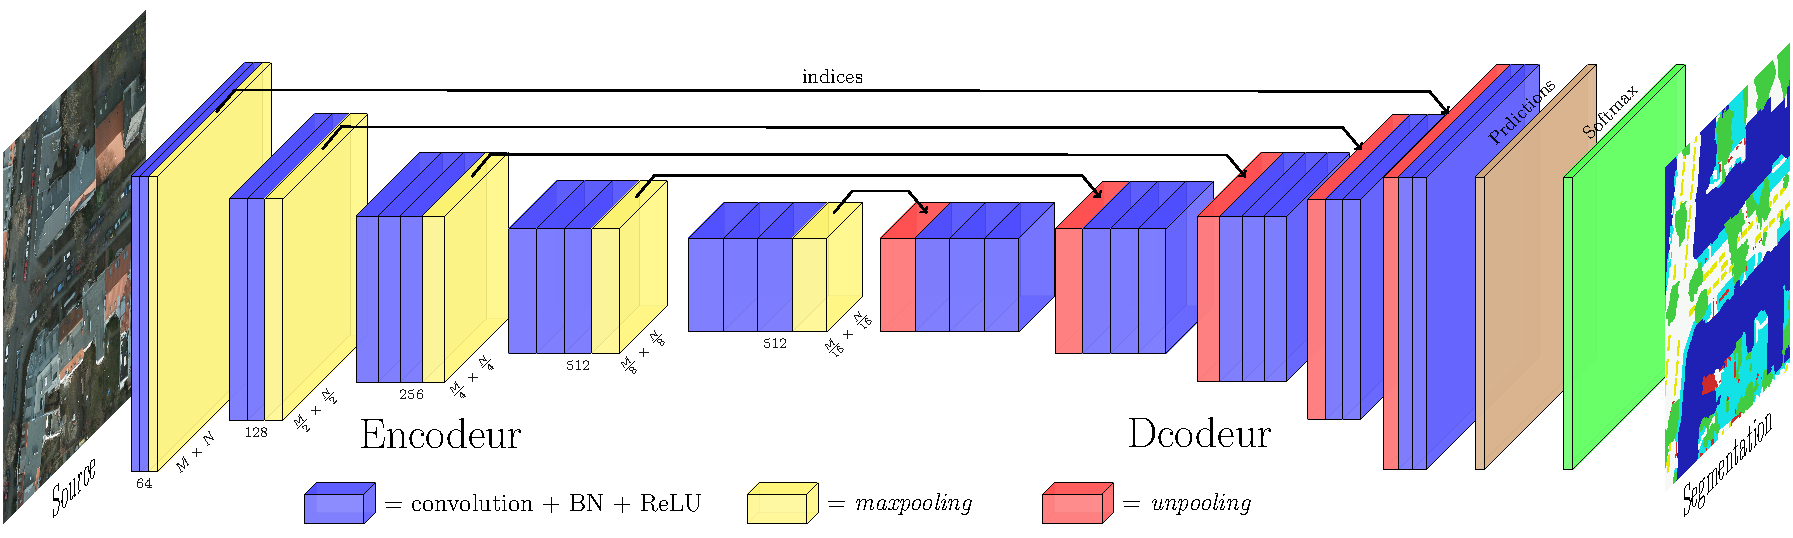
\includegraphics[width=4cm]{../../Manuscrit/Chapitre2/segnet.pdf}} node[below] {\large réseau profond} (1,0);
\node at (-0.5, -1) {\large de segmentation};

\node at (4, 0) {\includegraphics[width=4cm]{../../Publications/GEOBIA16/images/potsdam_vehicle_0_pred}};
\node at (4, -3) {\Large Carte sémantique};

\draw [ultra thick,->] (6.5, 0) -- node[above] {\large extraction} node[below] {\large des véhicules} (9.5,0);

\node at (12, 0) {\includegraphics[width=4cm]{../../Illustrations/potsdam_vehicle_0_gt_vehicles}};
\node at (12,-3) {\Large Masque des véhicules};

\draw [ultra thick,->] (14.5, 0) -- node[above] {\includegraphics[width=3.8cm]{../../Illustrations/tikz/alexnet.pdf}} node[below] {\large réseau profond} (17.5,0);
\node at (16, -1) {\large classification};

\node at (20, 0) {\includegraphics[width=4cm]{../../Publications/GEOBIA16/images/classif}};
\node at (20, -3) {\Large Véhicules classifiés};

\end{tikzpicture}
\end{document}

  }
  \caption{Illustration de la méthode \emph{segment-before-detect} pour la segmentation, détection et classification de véhicules.}
  \label{fig:pipeline}
\end{figure}

\subsubsection{Détection de petits objets}

Comme nous l'avons vu dans les sections précédentes, un réseau profond de type SegNet est suffisamment précis pour prédire des véhicules individuels dans des images haute résolution ($<\SI{50}{\centi\meter\px}$). Dans ce cas, il suffit alors de réaliser une extraction des composantes connectées pour obtenir les instances individuelles des véhicules présents dans l'image. Pour chaque composante connectée, le calcul de la boîte englobante l'entourant est alors immédiat.

Cependant, les prédictions issues de SegNet sont susceptibles d'être bruitées. En particulier, les \gls{CNN} appliqués à l'observation de la Terre tendent à produire des transitions inter-classes imprécises~\cite{marmanis_classification_2017}. Par conséquent, nous éliminons une grande partie des faux positifs et séparons les véhicules susceptibles d'avoir été prédits comme appartenant à la même composante connexe en appliquant une ouverture morphologique au masque sémantique obtenu par SegNet. Nous éliminons ensuite les objets dont la surface est inférieure à un seuil strict pour supprimer les fausses alarmes dues aux erreurs de segmentation, comme les bouches de ventilation sur les toits ou certains éléments du mobilier urbain. Bien que simple, nous allons voir que cette approche permet d'augmenter significativement les performances en détection de SegNet.

\subsubsection{Reconnaissance de véhicules par \gls{CNN}}

En admettant que nous sommes en mesure de localiser les véhicules, nous cherchons dès lors à en identifier le type. Ainsi, nous cherchons à déterminer si le véhicule est une voiture, un camion, une camionette, etc. Il s'agit d'un problème classique de reconnaissance d'objet que les \gls{CNN} peuvent aisément résoudre. Nous appliquons donc l'approche classique consistant à spécialiser~\cite{nogueira_towards_2016,zhou_deep_2016} un modèle de \gls{CNN} pré-entraîné sur la base de données ImageNet~\cite{russakovsky_imagenet_2015} pour la reconnaissance de véhicules.

Nous comparons en particulier les modèles les plus utilisés dans la littérature pour la classification de petites images ($\simeq$\SI{30x30}{\px}): LeNet~\cite{lecun_gradient-based_1998}, AlexNet~\cite{krizhevsky_imagenet_2012} et VGG-16~\cite{simonyan_very_2014}.

Notre objectif est d'entraîner ce classifieur sur une grande base de données de véhicules et de l'appliquer sur des données issues d'une scène spécifique. Nous risquons donc d'être confrontés au problème de surapprentissage. En effet, nous cherchons à transférer des connaissances d'un jeu à de données à un autre. Pour améliorer la généralisabilité du modèle, deux techniques peuvent être employées: l'adaptation de domaine et l'augmentation de données. L'adaptation de domaine cherche à minimiser les différence entre le jeu de donnée d'apprentissage et celui d'inférence. L'augmentation de données cherche quant à elle à générer de nouvelles images d'entraînement synthétiques pour améliorer la robustesse du classifieur.

Nous proposons ainsi de normaliser l'ensemble des véhicules pour que ceux-ci présentent le même azimuth, c'est-à-dire que toutes les images présentent un véhicule dont la direction principale est horizontale. Durant l'apprentissage, nous utilisons les boîtes englobantes pour estimer la direction principale du véhicule puis nous appliquons une rotation pour l'alignement. Durant l'inférence, nous utilisons la composante connectée du masque correspondant au véhicule pour réaliser cette opération.

Enfin, nous augmentons le jeu de données d'apprentissage en appliquant diverses opérations géométriques pour augmenter la variété des échantillons: translations ($\pm$\SI{10}{\px}), zooms (jusqu'à 1,25$\times$), rotations (90\degre, 180\degre and 270\degre) et symétries axiales, comme illustrées par la~\cref{fig:augmented_car}. Lorsque la stratégie de réalignement est utilisée, seule la rotation à 180\degre est appliquée.

\begin{figure}[t]
	\begin{subfigure}{0.142\textwidth}
    	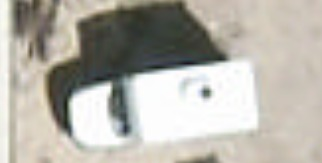
\includegraphics[width=\textwidth]{images/1}
        \caption*{identité}
    \end{subfigure}%
    \begin{subfigure}{0.142\textwidth}
    	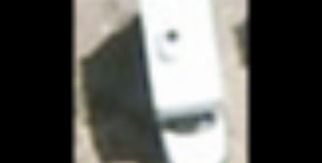
\includegraphics[width=\textwidth]{images/2}
        \caption*{rotation 90\degre}
    \end{subfigure}%
    \begin{subfigure}{0.142\textwidth}
    	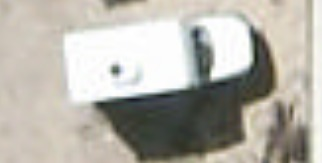
\includegraphics[width=\textwidth]{images/3}
        \caption*{rotation 180\degre}
    \end{subfigure}%
    \begin{subfigure}{0.142\textwidth}
    	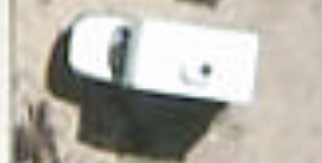
\includegraphics[width=\textwidth]{images/4}
        \caption*{sym. horizon.}
    \end{subfigure}%
    \begin{subfigure}{0.142\textwidth}
    	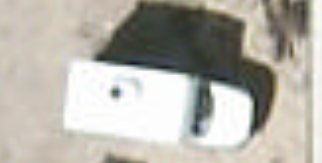
\includegraphics[width=\textwidth]{images/5}
        \caption*{sym. verticale}
    \end{subfigure}%
    \begin{subfigure}{0.142\textwidth}
    	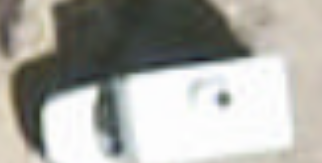
\includegraphics[width=\textwidth]{images/6}
        \caption*{zoom}
    \end{subfigure}%
    \begin{subfigure}{0.142\textwidth}
    	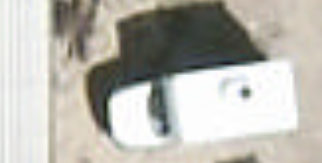
\includegraphics[width=\textwidth]{images/7}
        \caption*{translation}
    \end{subfigure}
    \caption{Augmentation de données sur un véhicule de la base \gls{VEDAI}.}
    \label{fig:augmented_car}
\end{figure}

\subsection{Segmentation de véhicules}

Afin d'entraîner un \gls{CNN} pour la classification de véhicules, nous devons utiliser une base d'apprentissage suffisamment grande. Pour ce faire, nous utilisons le jeu de données \gls{VEDAI}~\cite{razakarivony_vehicle_2016} (cf.~\cref{annexe:vedai}), contenant de nombreuses annotations de véhicules dans des images aériennes. \gls{VEDAI} est utilisé pour entraîner le \gls{CNN} que nous utilisons pour la reconnaissance de véhicules, qui sera appliqué en inférence sur le jeu de données \gls{ISPRS} Potsdam, noté Potsdam par la suite (cf.~\cref{annexe:isprs}). Les résultats sur \gls{VEDAI} sont obtenus par validation croisée en utilisant 2/3 des images pour l'entraînement et 1/3 pour l'inférence.

Afin de valider notre méthode, nous utilisons dans un premier temps le jeu de données \gls{ISPRS} Potsdam sur lequel nous avons manuellement annoté les véhicules dans quatre sous-catégories: voitures, vans, camions et pick-ups. Les véhicules ayant été initialement annotés dans la classe de rejet (engins de chantier, notamment) dans la vérité terrain originale ne sont pas pris en compte. Comme indiqué dans le~\cref{tab:vehicle_counts}, le jeu de données est largement dominé par les voitures (94\% des véhicules).

Nous entraînons un SegNet pour la segmentation sémantique sur ce jeu de données et nous appliquons le \gls{CNN} entraîné sur \gls{VEDAI} pour la reconnaissance de véhicules. Les résultats sont obtenus par validation croisée utilisant 18 tuiles pour l'entraînement et 6 tuiles pour la validation. La résolution spatiale est interpolée à \SI{12,5}{\centi\meter/\px} pour correspondre avec celle de \gls{VEDAI} au lieu des \SI{5}{\centi\meter/\px} initiaux.

Dans un second temps, nous utilisons le jeu de données NZAM/ONERA Christchurch, noté Christchurch par la suite (cf.~\cref{annexe:christchurch}). Pour rappel, la vérité terrain de ce jeu de données est moins précise que celle de Potsdam, mais se rapproche plus des annotations par boîte englobante habituellement disponibles en détection. Nous étendons également cette vérité terrain en déclinant les véhicules en quatre types: voitures, camions, vans et pick-ups. À nouveau, le jeu de données est dominé par la classe voiture~\cref{tab:vehicle_counts}.

Le jeu de données NZAM/ONERA Christchurch contenant seulement des polygones englobants, susceptibles de s'intersecter, pour les arbres, les bâtiments et les véhicules, nous transformons ces annotations en cartes sémantiques. Pour ce faire, nous définissons quatre classes d'intérêt: arrière-plan, bâtiments, végétation et véhicules. Nous construisons la vérité terrain dense en étiquetant d'abord les pixels appartenant à une boîte englobante de bâtiment, puis ceux appartenant à des véhicules et finalement à la végétation. Les pixels restants sont étiquetés comme arrière-plan. Cet ordre permet de prendre en compte la présence de certains véhicules sur des parkings en toit de bâtiment et la présence de végétation arborescente pouvant masquer certaines voitures. Pour prendre en compte l'incertitude sur les boîtes englobantes, les pixels appartenant à un disque de rayon \SI{5}{\px} autour des frontières sont ignorés.

Nous entraînons un SegNet pour la segmentation sémantique sur ce jeu de données et nous appliquons le \gls{CNN} entraîné sur \gls{VEDAI} pour la reconnaissance de véhicules. Les résultats sont obtenus par validation croisée utilisant 3 tuiles pour l'entraînement et 1 tuile pour la validation. La résolution spatiale est interpolée à \SI{12,5}{\centi\meter/\px} pour correspondre avec celle de \gls{VEDAI} au lieu des \SI{10}{\centi\meter/\px} initiaux.

\begin{figure}[t]
\centering
	\begin{subfigure}[]{0.45\textwidth}
    	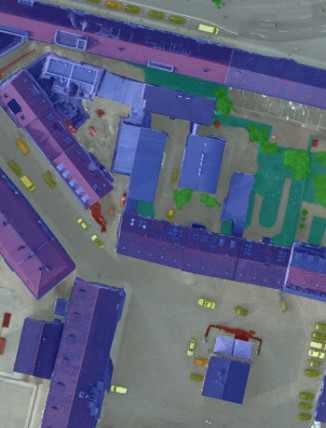
\includegraphics[angle=90,width=\textwidth]{images/potsdam_illu}
      \caption{ISPRS Potsdam}
    \end{subfigure}
    \begin{subfigure}[]{0.45\textwidth}
    	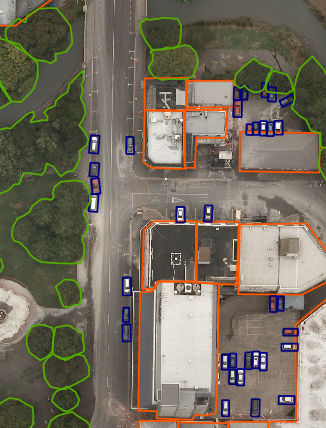
\includegraphics[angle=90,width=\textwidth]{images/christchurch_illu}
      \caption{NZAM/ONERA Christchurch}
    \end{subfigure}
    \caption{Exemples d'annotations dans les jeux de données considérés.}
    \label{fig:datasets}
\end{figure}
\unskip
\begin{table}[t]
	\setlength\tabcolsep{2.5pt}
    \caption{Nombre de véhicules par classe dans les différents jeux de données.}
    \label{tab:vehicle_counts}
    \scalebox{0.9}[0.9]{
	\begin{tabularx}{1.1\textwidth}{Y c c c c c c c cc}
    \toprule
    \textbf{Jeu de données} & \textbf{Voiture} & \textbf{Camion} & \textbf{Van} & \textbf{Pick-up} & \textbf{Bateau} & \textbf{Camping-car} & \textbf{Autres} & \textbf{Avion} & \textbf{Tracteur}\\
    \midrule
    VEDAI & 1340 &  300 & 100 & 950 & 170 & 390 & 200 & 47 & 190\\
    ISPRS Potsdam & 1990 & 33 & 181 & 40 & - & - & - & - & -\\
    NZAM/ONERA Christchurch & 2267 & 73 & 120 & 90 & - & - & - & - & -\\
    \bottomrule
    \end{tabularx}}
\end{table}

\subsubsection{Segmentation sémantique}
\begin{figure}[t]
	\centering
	\begin{subfigure}{0.3\textwidth}
    	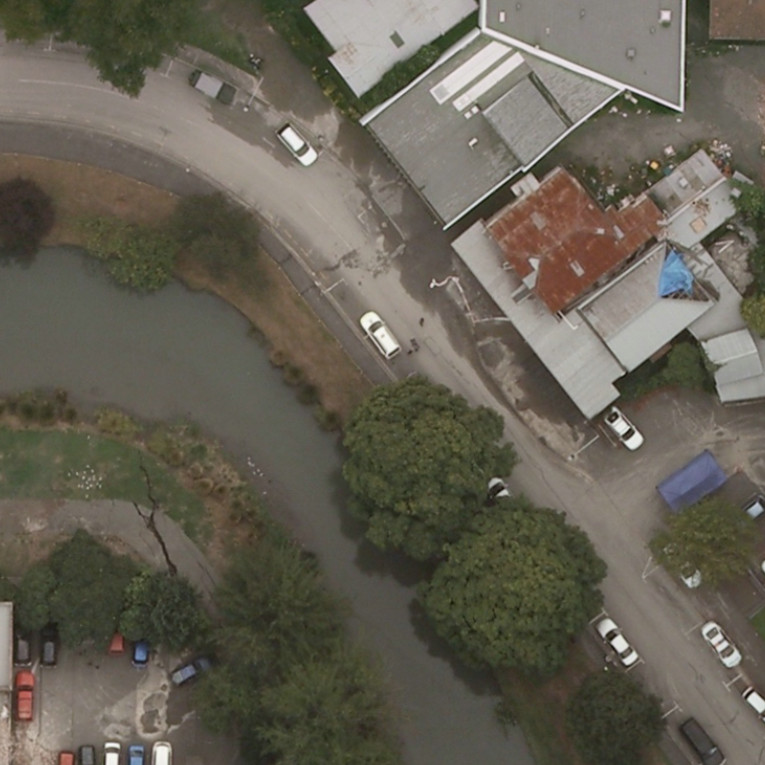
\includegraphics[width=\textwidth]{images/christchurch_extract_rgb}
      \caption*{\glssymbol{RVB} (Christchurch)}
    \end{subfigure}
    \begin{subfigure}{0.3\textwidth}
    	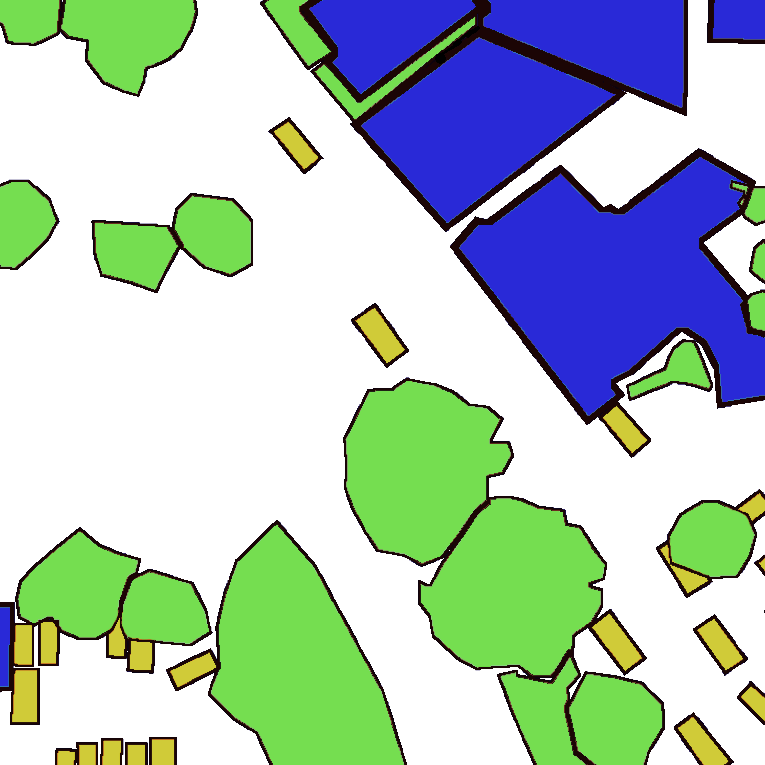
\includegraphics[width=\textwidth]{images/christchurch_extract_gt}
      \caption*{Vérité terrain (Christchurch)}
    \end{subfigure}
    \begin{subfigure}{0.3\textwidth}
    	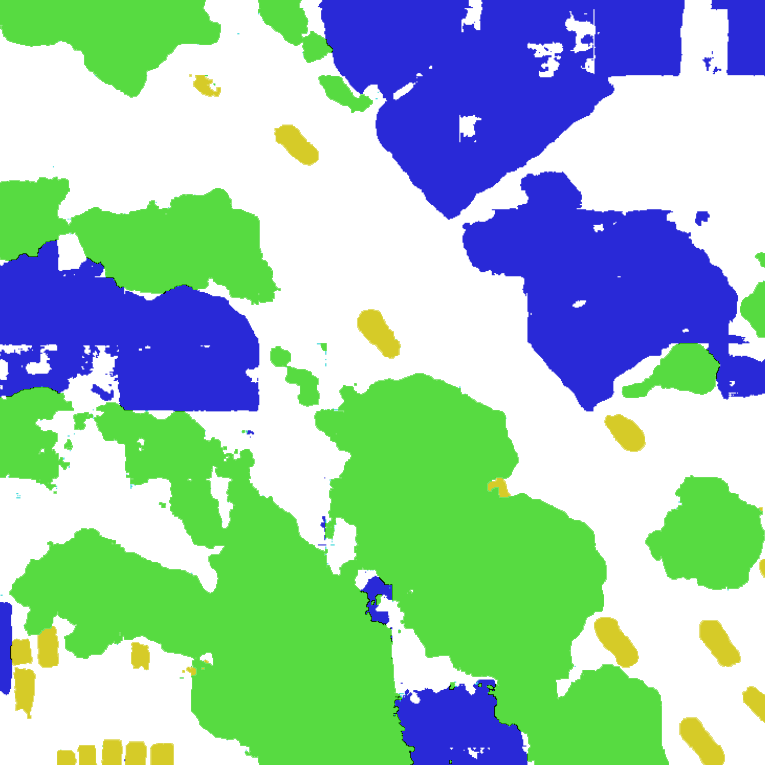
\includegraphics[width=\textwidth]{images/christchurch_extract_pred}
      \caption*{SegNet (Christchurch)}
    \end{subfigure}\\
    	\begin{subfigure}{0.3\textwidth}
    	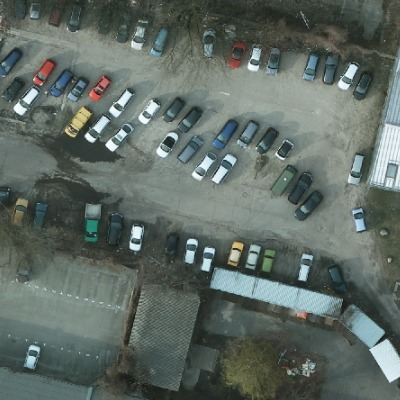
\includegraphics[width=\textwidth]{images/parking_zoom_rgb}
        \caption*{\glssymbol{RVB} (Potsdam)}
    \end{subfigure}
    \begin{subfigure}{0.3\textwidth}
    	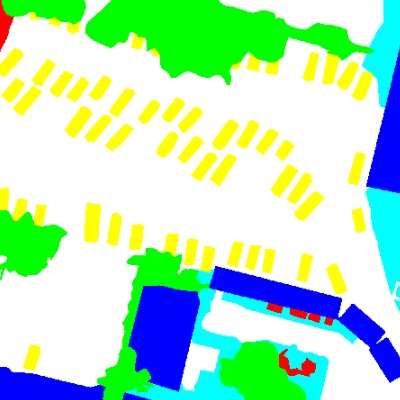
\includegraphics[width=\textwidth]{images/parking_zoom_gt}
        \caption*{Vérité terrain (Potsdam)}
    \end{subfigure}
    \begin{subfigure}{0.3\textwidth}
    	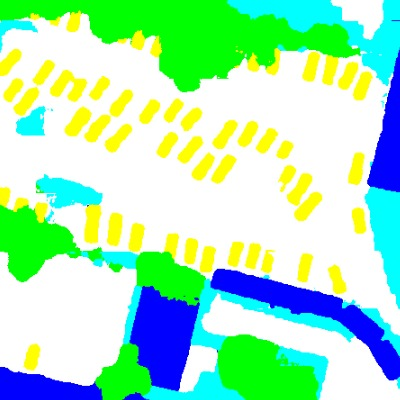
\includegraphics[width=\textwidth]{images/parking_zoom_pred}
        \caption*{SegNet (Potsdam)}
    \end{subfigure}

    \caption{Exemples de segmentation obtenues sur Potsdam et Christchurch.\\\isprslegende}
    \label{fig:segmentations}
\end{figure}

Nous détaillons dans le~\cref{table:potsdam_seg} les scores $F_1$ et l'exactitude globale du SegNet entraîné sur Potsdam. Il est important de noter que les résultats obtenus à résolution de \SI{12,5}{\centi\meter/\px} sont similaires à ceux obtenues à \SI{5}{\centi\meter/\px}. Un exemple qualitatif de segmentation est illustré dans la~\cref{fig:segmentations}.

\begin{table}[t]
\centering
	\caption{Résultats de segmentation sémantique sur le jeu de données \gls{ISPRS} Potsdam (scores $F_1$ et exactitude globale).}
    \label{table:potsdam_seg}
    %\setlength{\tabcolsep}{2pt}
    \scalebox{0.8}[0.8]{
	\begin{tabularx}{1.25\textwidth}{Yccccccc}
 	  \toprule
    \textbf{Jeu de données }&\textbf{ Méthode} & \textbf{Routes} & \textbf{Bâtiments} & \textbf{Vég. basse} & \textbf{Arbres} & \textbf{Véhicules} & \textbf{Exactitude}\\
    \midrule
    Validation \SI{12,5}{\centi\meter/\px} & SegNet \glssymbol{RVB} & \res{92.4}{0.6} & \res{95.8}{1.9} & \res{85.8}{1.3} & \res{83.0}{2.1} & \res{95.7}{0.3} & \res{90.6}{0.6}\\
    \midrule
    \multirow{3}{*}{Test \SI{5}{\centi\meter/\px}} & SegNet \glssymbol{IRRV} & 92.4\% & 95.8\% & \textbf{86.7\%} & 87.4\% & \textbf{95.1\%} & \textbf{90.0\%}\\
     & \glsname{FCN} + \glsname{CRF}~\cite{sherrah_fully_2016} & 91.8\% & 95.9\% & 86.3\% & 87.7\% & 89.2\% & 89.7\%\\
     & ResNet-101~\cite{liu_context-aware_2017} & \textbf{92.8\%} & \textbf{96.9\%} & 86.0\% & \textbf{88.2\%} & 94.2\% & 89.6\%\\
     \bottomrule
  \end{tabularx}}
\end{table}

Comme illustré dans la~\cref{table:christchurch_seg}, un SegNet entraîné sur NZAM/ONERA Christchurch atteint 61.9\% d'exactitude pixel à pixel sur les véhicules, ce qui est acceptable compte-tenu de la grossiereté des annotations en comparaison de celles de Potsdam. Ce constat est intéressant dans la mesure où il prouve qu'il est possible d'apprendre des modèles de segmentation sémantique, même en présence de simples boîtes englobantes originellement prévues pour entraîner des détecteurs. L'inférence sur une tuile de Christchurch nécessite environ 120 secondes sur un \gls{GPU} NVIDIA Tesla K20c. Un exemple de segmentation est illustré dans la~\cref{fig:segmentations}.

\begin{table}[t]
\centering
	\caption{Résultats de segmentation sémantique sur NZAM/ONERA Christchurch (scores $F_1$ et exactitude globale).}
    \label{table:christchurch_seg}
	\begin{tabular}{cccccc}
 	\toprule
    \textbf{} & \textbf{Arrière-plan} & \textbf{Bâtiments} & \textbf{Végétation} & \textbf{Véhicules} & \textbf{Exactitude}\\
    \midrule
    \glsname{RVB} & 75.6\% $\pm$ 8.9 & 91.7\% $\pm$ 1.3 & 55.2\%  $\pm$ 11.6 & 61.9\%  $\pm$ 2.4 & 84.4\%  $\pm$ 2.6\\
    \bottomrule
    \end{tabular}
\end{table}

\subsection{Détection de véhicules}
\begin{figure}[t]
\centering
	\begin{subfigure}{0.3\textwidth}
    	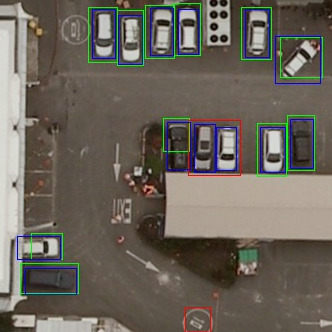
\includegraphics[width=\textwidth]{images/christchurch_draw1}
    	\caption{}
    \end{subfigure}
    \begin{subfigure}{0.3\textwidth}
    	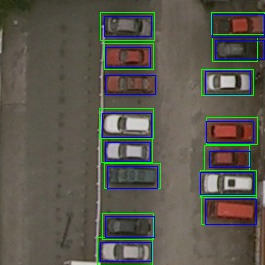
\includegraphics[width=\textwidth]{images/christchurch_draw2}
    	\caption{}
    \end{subfigure}\begin{subfigure}{0.3\textwidth}
    	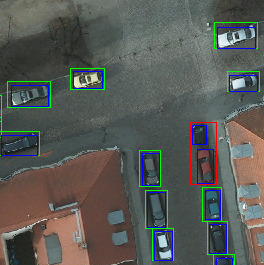
\includegraphics[width=\textwidth]{images/potsdam_draw1}
    	\caption{}
    \end{subfigure}\vspace{-12pt}
	\caption{Exemples de détections sur Potsdam et Christchurch (vrais positifs en vert, faux positifs en rouge et vérité terrain en bleu). (\textbf{a}) Christchurch; (\textbf{b}) Christchurch; (\textbf{c}) Potsdam.}
    \label{fig:detection_samples}
\end{figure}

Nous appliquons sur les deux jeux de données une ouverture morphologique d'un rayon de \SI{3}{\px} ($\simeq$ \SI{35}{\centi\meter} d'incertitude sur les formes de véhicules prédites) pour isoler des véhicules ayant pu être prédits dans la même composante connexe. Nous supprimons également les composantes connexes couvrant moins de \SI{1,5}{\meter\squared} (\SI{100}{\px}). Une voiture citadine couvre environ \SI{4}{\meter\squared}, et nous considérons que donc les occlusions peuvent recouvrir jusqu'à 60\% du véhicule. Nous extrayons ensuite les composantes connexes dans le masque des véhicules et nous calculons la boîte englobante de chaque composante. Pour le jeu de données \gls{ISPRS} Potsdam, comme la vérité terrain initiale est constituée d'annotations pixelliques denses, nous avons régressé une boîte englobante pour chaque composante connectée en corrigeant manuellement les rares erreurs.

Nous suivons les pratiques habituelles en détection d'objet~\cite{everingham_pascal_2014} et nous définissons un vrai positif comme une boîte englobante prédite dont l'intersection sur union avec une boîte englobante de la vérité terrain dépasse 0,5. Si plusieurs prédictions existent pour le même véhicule, nous conservons celle avec la plus haute valeur d'\gls{IsU}. Les autres prédictions sont considérées comme des fausses alarmes. Sur le jeu de données NZAM/ONERA Christchurch, nous comparons nos résultats sur la même tuile que celle choisie par~\citet{randrianarivo_contextual_2016}, qui ont appliqué un \emph{Discriminatively trained Model Mixture} (DtMM) contenant cinq modèles, un pour chaque orientation principale.

Pour évaluer l'effet de l'ouverture morphologique sur les performances en segmentation d'instance, nous détaillons dans le~\cref{table:morpho_results} la moyenne de l'\gls{IsU} calculée sur les instances de véhicules et les scores précision/rappel finaux en fonction des divers pré-traitements appliqués. Ceci montre que la simple ouverture morphologique et l'élimination des véhicules candidats dont la surface est inférieure à 100px permet de grandement améliorer les performances en éliminant les faux positifs. Ceci est particulièrement vrai pour le jeu de données NZAM/ONERA dans lequel les annotations grossières conduisent à des cartes sémantiques imprécises après inférence. Le processus complet atteint un score \gls{IsU} de plus de 74\% sur Potsdam et plus de 70\% sur Christchurch.

Finalement, nous indiquons les résultats de détection dans le~\cref{table:detection_results}. Sur NZAM/ONERA Christchurch, notre méthode \textit{segment-before-detect} obtient des résultats significativement supérieurs aux approches par mélange de modèles et \gls{HOG}+\gls{SVM}. Bien qu'aucune autre méthode de détection de véhicules n'ait été appliquée sur Potsdam, nous indiquons également nos scores de précision/rappel sur ce jeu de données. Des exemples qualitatifs de détection sont présentés dans la~\cref{fig:detection_samples}.

 Sur Christchurch, où les annotations sont grossières, le score $F_1$ atteint $0,81$, tandis qu'il dépasse $0,87$ sur Potsdam. En comparaison, l'approche classique par modèles déformables~\cite{randrianarivo_urban_2013} n'atteint qu'un score $F_1$ de seulement $0,74$. Notons par ailleurs que nous indiquons nos résultats pour lesquels un vrai positif est défini comme ayant un score \gls{IsU} d'au moins $0,5$. Dans la littérature, à des résolutions similaires ($<\SI{30}{\centi\meter}$), la majorité des travaux considèrent qu'un vrai positif sur des véhicules de cette taille correspond à un seuil de $0,25$. Ainsi, sur un jeu de données similaire, \citet{tang_vehicle_2017} obtiennent un score $F_1$ de $0,83$ en utilisant le réseau de détection d'objets Faster-RCNN~\cite{ren_faster_2017}. De façon postérieure à nos travaux, \citet{van_etten_you_2018} introduit un jeu de données de détection de véhicules à des résolutions équivalentes (entre \SI{10}{\centi\meter} et \SI{1}{\meter}) et adapte le réseau YOLO~\cite{redmon_you_2016} pour l'imagerie aérienne. Ils parviennent ainsi obtenir un score $F_1$ d'environ $0,90$ et à prédire le nombre de véhicules avec une erreur relative de 5\%. Toutefois, leur approche ne prédit d'une part que des boîtes englobantes et le seuil considéré pour le score $F_1$ est fixé à 0,25, ce qui est bien plus permissif que celui que nous avons choisi. Dans l'ensemble, l'approche de segmentation avant détection paraît très compétitive avec les méthodes de détection pure, et permet d'extraire les instances d'objet bien plus finement en inférant des formes plutôt que des boîtes englobantes.


\begin{table}[t]
\centering
  \caption{Segmentation d'instance et détection de véhicules pour différents pré-traitements morphologiques (\gls{IsU} moyen, précision et rappel).}
  \label{table:morpho_results}
  \begin{tabularx}{\textwidth}{Y c c c c}
  \toprule
  \textbf{Jeu de données} & \textbf{Pré-traitement} & \textbf{\gls{IsU} moyen} & \textbf{Précision} & \textbf{Rappel}\\
  \midrule
  %\multirow{3}{*}{Potsdam} & AlexNet & 81\% & 42\% & \textbf{50\%} & \textbf{50\%} & 75\% & 56\%\\
  %& VGG & 83\% & 55\% & \textbf{50\%} & 33\% & 77\% & 55\%\\
  %& AlexNet+R & \textbf{99\%} & \textbf{66\%} & 25\% & 0\% & \textbf{83\%} & 48\%\\
  \multirow{3}{*}{\shortstack{NZAM/ONERA\\ Christchurch}} & $\emptyset$ & 60.0\% & 0.597 & 0.797\\
  & Ouverture & 69.8\% & 0.817 & 0.791\\
  & Ouverture + retrait des petits objets & 70.7\% & 0.833 & 0.791\\
  \midrule
  \multirow{3}{*}{ISPRS Potsdam} & $\emptyset$ & 70.1\% & 0.748 & 0.842\\
  & Ouverture & 73.3\% & 0.866 & 0.842\\
  & Ouverture + retrait des petits objets & 74.2\% & 0.907 & 0.841\\
  \bottomrule
  \end{tabularx}
\end{table}
\unskip
\begin{table}[t]
\centering
  \caption{Résultats de détection de véhicules sur Potsdam et Christchurch.}
  \label{table:detection_results}
  \begin{tabular}{cccc}
  \toprule
  \textbf{Jeu de données} & \textbf{Méthode} & \textbf{Précision} & \textbf{Rappel}\\
  \midrule
  %\multirow{3}{*}{Potsdam} & AlexNet & 81\% & 42\% & \textbf{50\%} & \textbf{50\%} & 75\% & 56\%\\
  %& VGG & 83\% & 55\% & \textbf{50\%} & 33\% & 77\% & 55\%\\
  %& AlexNet+R & \textbf{99\%} & \textbf{66\%} & 25\% & 0\% & \textbf{83\%} & 48\%\\
  \multirow{3}{*}{NZAM/ONERA Christchurch} & HOG+SVM~\cite{michel_local_2011} & 0.402 & 0.398\\
  & \emph{DtMM} (5 modèles)~\cite{randrianarivo_contextual_2016} & 0.743 & 0.737\\
  & \emph{Segment-before-detect} & \textbf{0.833} & \textbf{0.791}\\
  \midrule
  ISPRS Potsdam & \emph{Segment-before-detect} & 0.907 & 0.841\\
  \bottomrule
  \end{tabular}
\end{table}

Christchurch est un jeu de données plus complexe pour deux raisons. Tout d'abord, la densité de véhicules y est nettement plus élevée que pour Potsdam, la ville comprenant de nombreux véhicules resserrés sur des surfaces réduites. Ensuite, les annotations grossières empêchent le \gls{FCN} de prédire correctement les frontières des objets constituant la scène, ce qui conduit à des masques de véhicules imprécis (cf. \cref{fig:segmentations}, l'\gls{IsU} moyen sur Christchurch atteint 66.6\% contre plus de 80\% pour Potsdam). Cette combinaison rend le problème d'extraction des instances de véhicules plus difficile, mais reste toutefois à la portée de notre approche. Cependant, les boîtes englobantes obtenues tendent à couvrir plusieurs véhicules .
En dépit de cela, il est intéressant de constater que les résultats de segmentation sémantique sont relativement corrects, alors même que les annotations initiales étaient prévues pour la détection d'objet. Ainsi, la segmentation peut être utilisée comme étape intermédiaire pour des tâches de détection, pour lesquelles l'état de l'art nécessite des approches sophistiquées et complexes. L'étape d'extraction de composantes connectées pourrait en outre être améliorée en utilisant une extraction de boîte englobante plus robuste, soit par des approches morphologiques comme un \emph{watershed} appliqué aux cartes de probabilités~\cite{beucher_morphological_1993,bai_deep_2017}, soit en intégrant la prédiction d'instance au sein du réseau~\cite{dai_instance-aware_2015,he_mask_2017}.

\subsubsection{Estimation de la densité de véhicules}

Une fois les véhicules extraits des images, une tâche simple à réaliser consiste à estimer leur nombre sur une zone donnée. Nous divisons les deux jeux de données en cellule de $1000\times1000$px (soit $125\times$\SI{125}{\meter\squared}) et nous comparons le nombre de véhicules prédits au nombre de véhicules contenus dans la vérité terrain:
\begin{equation}
\frac{|\text{nombre de véhicules prédits} - \text{nombre réel de véhicules}~|}{\text{nombre réel de véhicules}}~~.
\end{equation}

Les résultats sont moyennés et arrondis à l'entier le plus proche pour chaque jeu de données et détaillés dans le~\cref{table:results_counting}. Sur Potsdam comme Christchurch, les estimations sont justes avec moins de 10\% d'erreur ($\pm$5 véhicules en moyenne). Les estimations sur Christchurch ont une erreur légèrement supérieure en raison de la segmentation et des détections moins précises.

\begin{table}[t]
\centering
  \caption{Erreur moyenne d'estimation du nombre de véhicules par cellule de 125$\times$\SI{125}{\meter\squared}.}
  \label{table:results_counting}
  \begin{tabularx}{\textwidth}{Ycc}
  \toprule
  \textbf{Dataset} & \textbf{ISPRS Potsdam} & \textbf{NZAM/ONERA Christchurch}\\
  \midrule
  Erreur absolue (erreur moyenne/total dans la vérité terrain) & 3/52 & 6/66\\
  Erreur relative & 7.9\% & 9.1\%\\
  \bottomrule
  \end{tabularx}
\end{table}

\begin{figure}[h]
  \centering
  \begin{subfigure}{0.34\textwidth}
    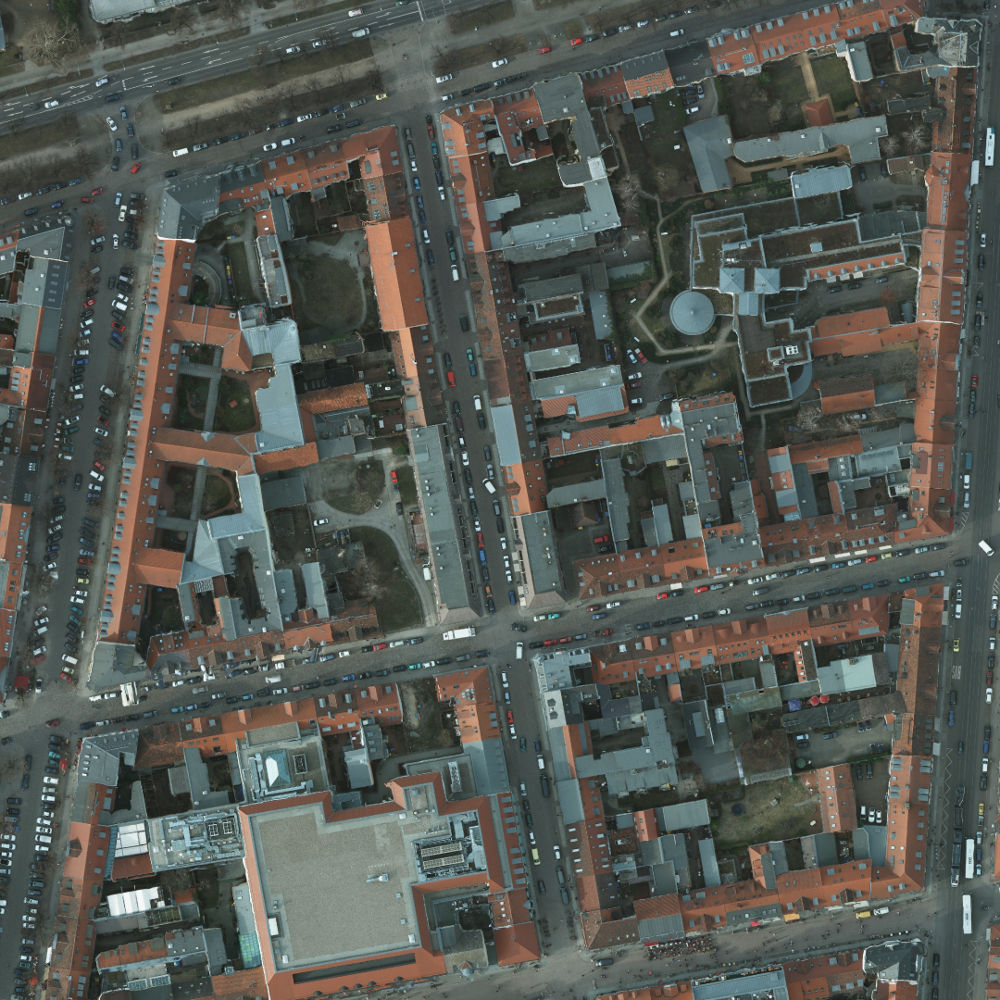
\includegraphics[width=\textwidth]{images/potsdam_vehicle_3_rgb}
    \caption{Image \glsname{RVB}}
  \end{subfigure}
  \hspace{0.1\textwidth}
  \begin{subfigure}{0.34\textwidth}
    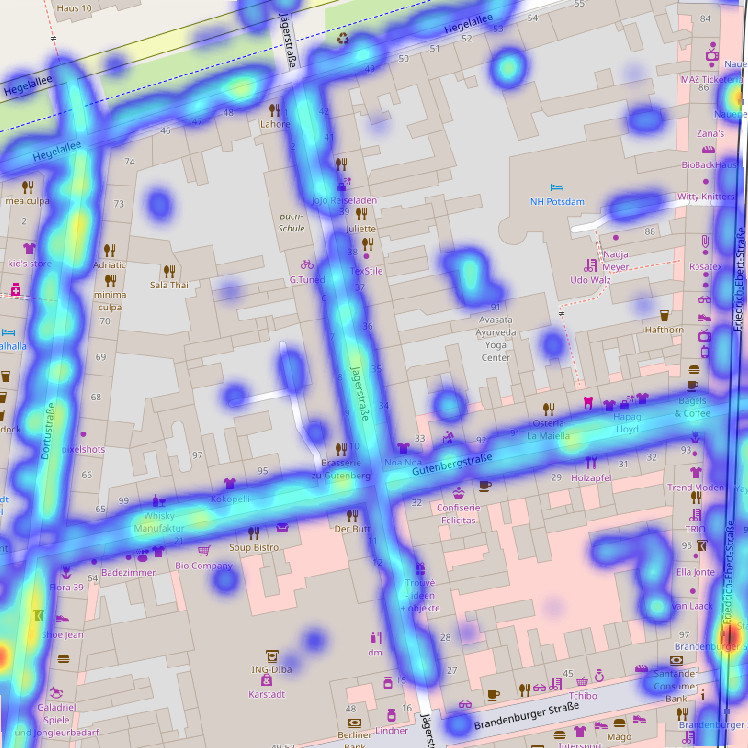
\includegraphics[width=\textwidth]{images/potsdam_vehicle_3_osm_dense}
    \caption{Densité de véhicules (Potsdam)}
  \end{subfigure}
  \begin{subfigure}{0.34\textwidth}
    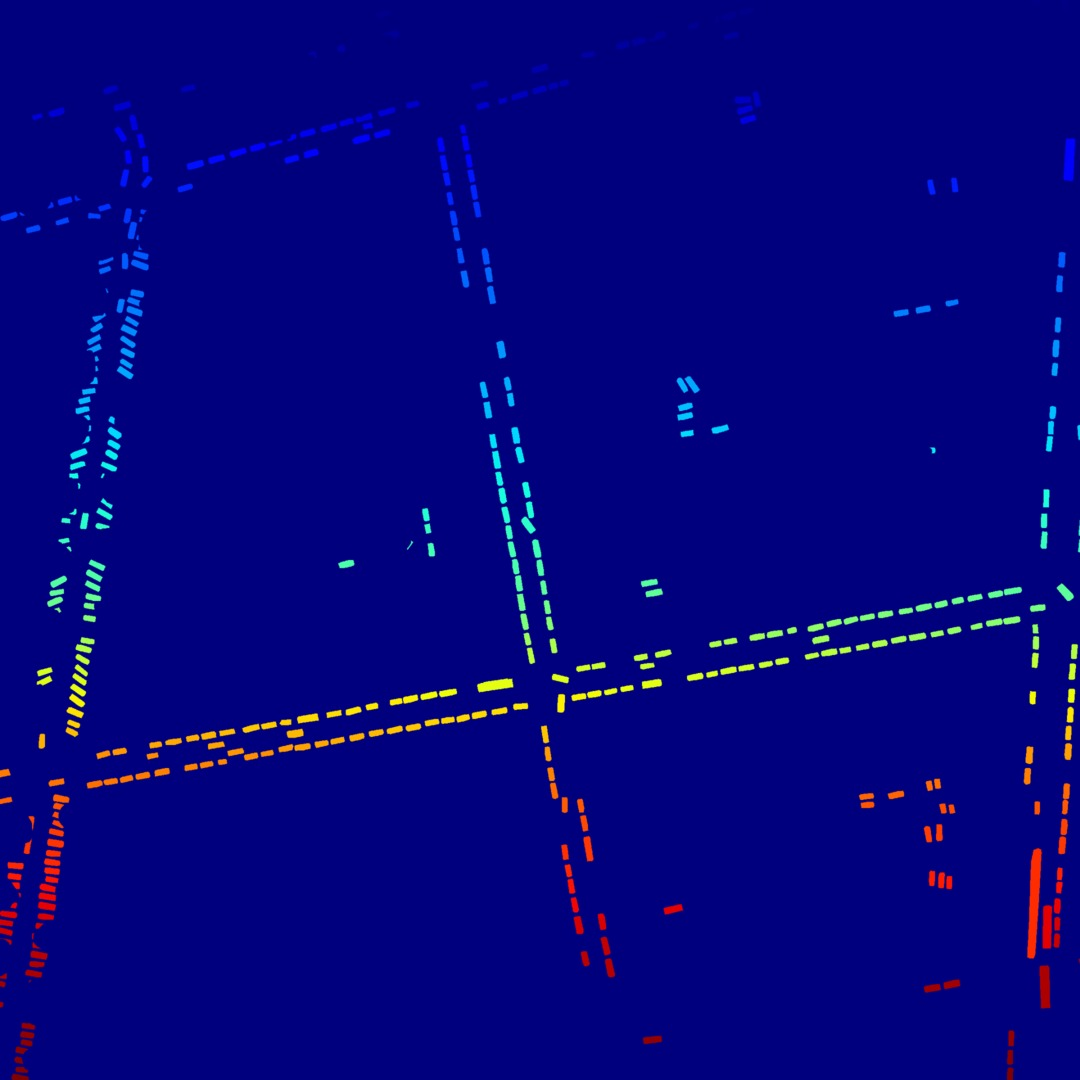
\includegraphics[width=\textwidth]{images/potsdam_vehicle_3_gt_vehicles}
    \caption{Vérité terrain (Potsdam)}
  \end{subfigure}
  \hspace{0.1\textwidth}
  \begin{subfigure}{0.34\textwidth}
    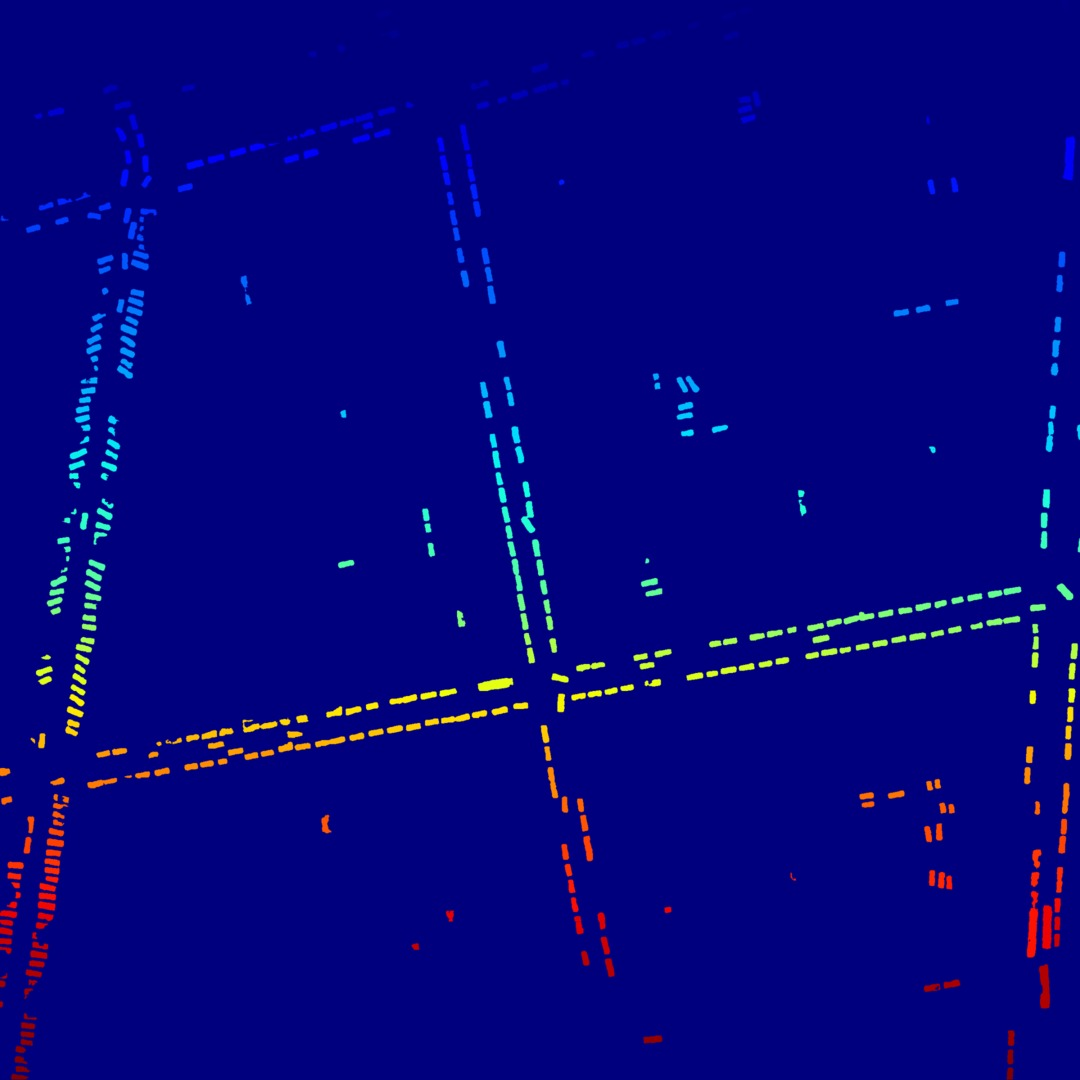
\includegraphics[width=\textwidth]{images/potsdam_vehicle_3_pred_vehicles}
    \caption{Véhicules prédits (Potsdam)}
  \end{subfigure}
  \caption{Visualisation des véhicules présents sur une des tuiles du jeu de données ISPRS Potsdam.}
  \label{fig:vehicle_density_maps}
\end{figure}

\begin{figure}[h]
  \centering
  \begin{subfigure}{0.35\textwidth}
    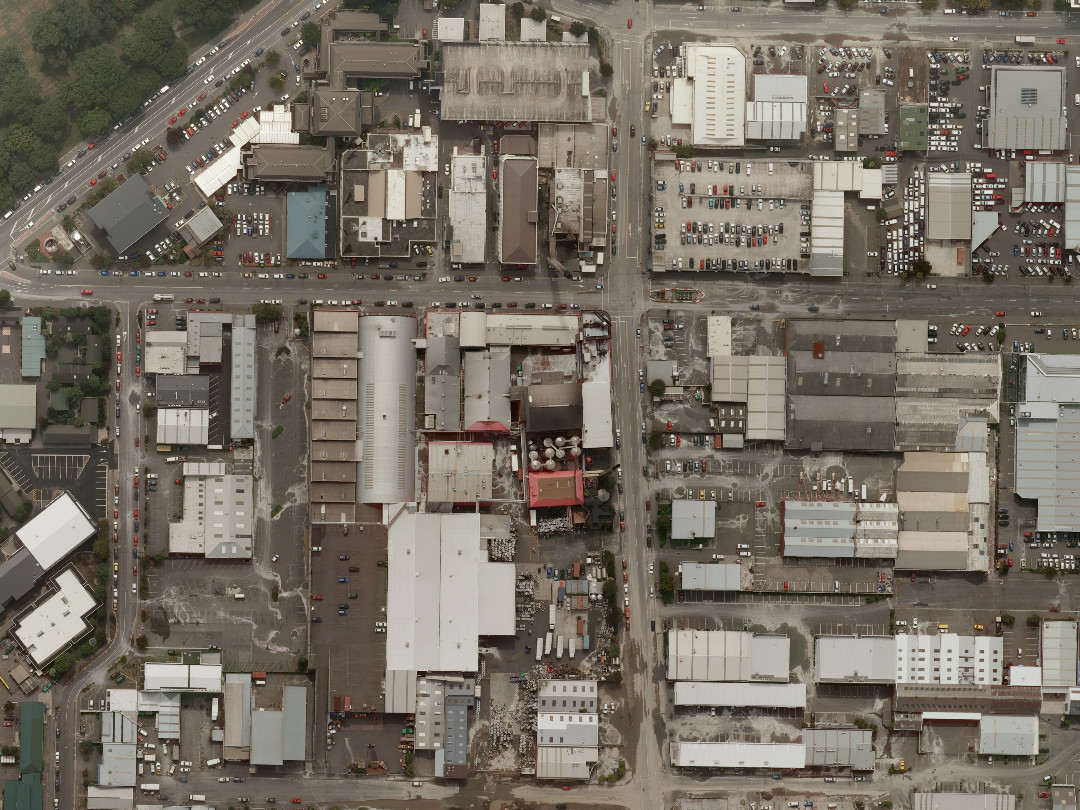
\includegraphics[width=\textwidth]{images/christchurch_vehicle_0_rgb}
    \caption{Image \glsname{RVB}}
  \end{subfigure}
  \hspace{0.1\textwidth}
  \begin{subfigure}{0.35\textwidth}
    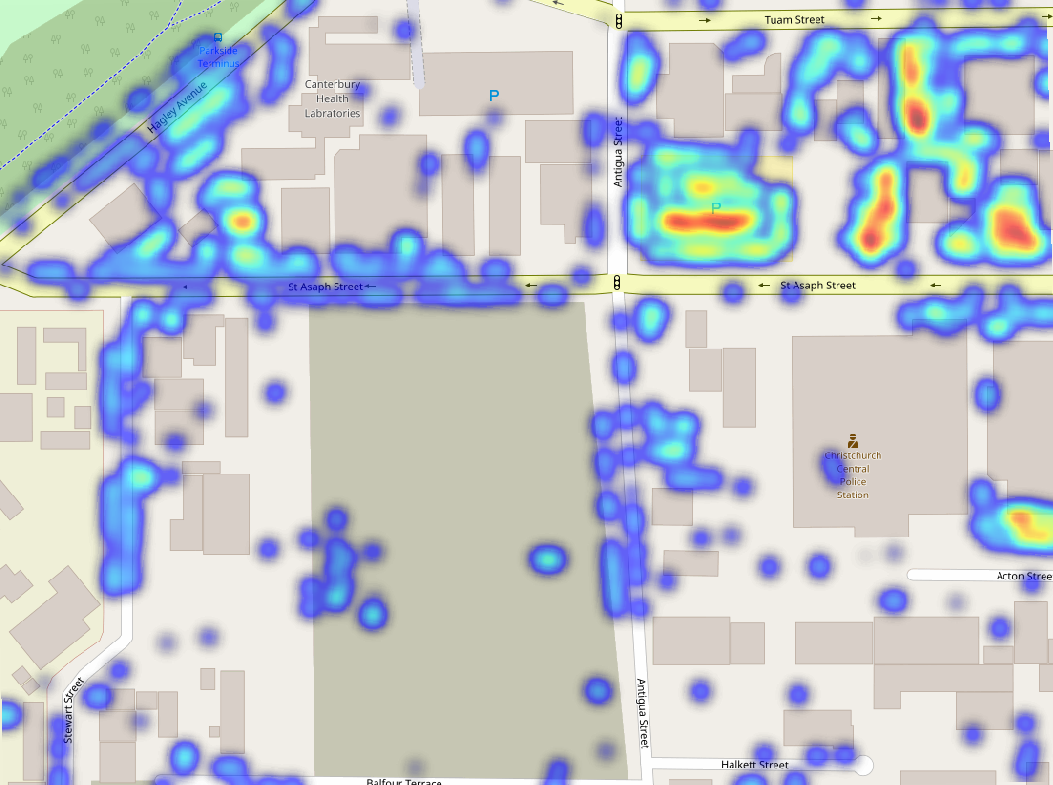
\includegraphics[width=\textwidth]{images/christchurch_vehicle_0_osm_vehicles_dense}
    \caption{Densité de véhicules (Christchurch)}
  \end{subfigure}\\
  \begin{subfigure}{0.35\textwidth}
    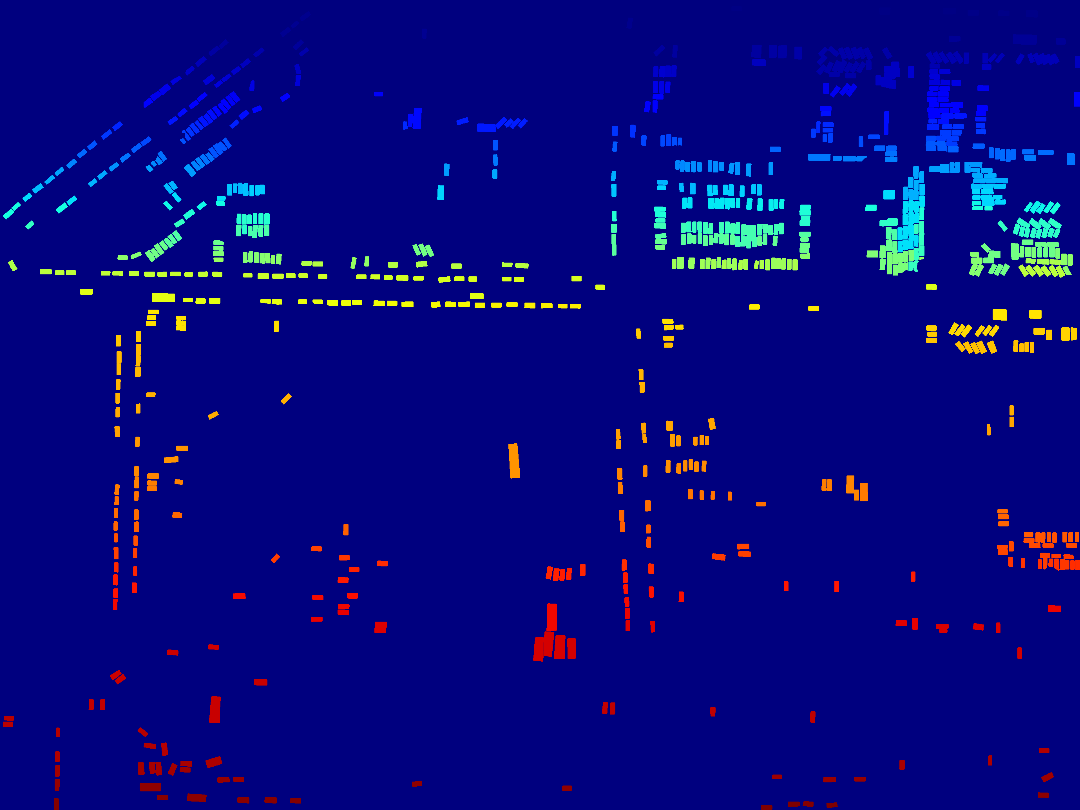
\includegraphics[width=\textwidth]{images/christchurch_vehicle_0_gt_vehicles}
    \caption{Vérité terrain (Christchurch)}
  \end{subfigure}
  \hspace{0.1\textwidth}
  \begin{subfigure}{0.35\textwidth}
    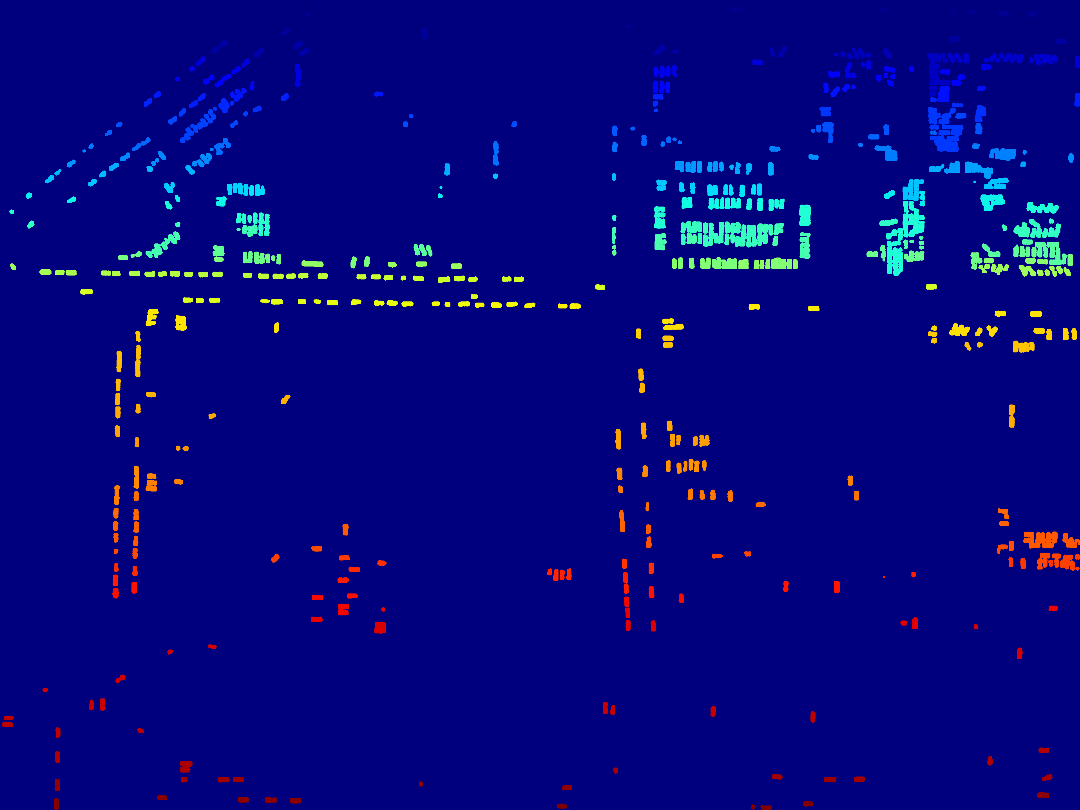
\includegraphics[width=\textwidth]{images/christchurch_vehicle_0_pred_vehicles}
    \caption{Véhicules prédits (Christchurch)}
  \end{subfigure}
  \caption{Visualisation des véhicules présents sur une des tuiles du jeu de données NZAM/ONERA Christchurch.}
  \label{fig:vehicle_density_maps_christchurch}
\end{figure}

Une fois ce type de densité calculée, il est possible de réduire la taille des cellules et de produire des cartes de densité de présence de véhicules, comme illustrées dans les\cref{fig:vehicle_density_maps,fig:vehicle_density_maps_christchurch}. Ce type de cartes de densité peut ensuite être intégré à des \gls{SIG} comme OpenStreetMap pour identifier automatiquement des routes encombrées, des parkings~\cite{kamenetsky_aerial_2015}, etc.

\subsection{Classification de véhicules}

Afin de classifier les véhicules identifiés, nous souhaitons utiliser un \gls{CNN}. Nous comparons trois architectures de complexité croissante: LeNet~\cite{lecun_gradient-based_1998}, AlexNet~\cite{krizhevsky_imagenet_2012} et VGG-16~\cite{simonyan_very_2014}.

 LeNet-5 est un petit \gls{CNN} que nous entraînons à partir d'une initialisation aléatoire sur les véhicules de \gls{VEDAI} en utilisant des images de dimensions $32\times32$. AlexNet et VGG-16 sont deux réseaux ayant gagné la compétition \gls{ILSVRC} en 2012 et 2014. Des expériences préliminaires montrent que l'utilisation des poids de ces réseaux pré-entraînés sur ImageNet permet d'augmenter de 10\% l'exactitude des modèles, ce qui est cohérent avec la littérature~\cite{nogueira_towards_2016,penatti_deep_2015}. Par conséquent, ces \gls{CNN} seront simplement spécialisés sur des images de véhicules à résolution $224 \times 224$ et $227 \times 227$.
 Ces tailles d'images permettent de conserver les poids pré-entraînés des couches entièrement connectées. En pratique, les véhicules issues des images aériennes auront une taille d'environ $25\times 25$. Nous extrayons donc des imagettes centrées sur ces véhicules incluant un contexte spatial de \SI{16}{\px} dans toutes les directions, cette approche ayant donné les meilleurs résultats. Un contexte plus large risquerait d'inclure d'autres véhicules dans la même imagette tandis qu'un contexte plus restreint diminue la quantité d'information disponible pour la classification. Les imagettes sont ensuites redimensionnées par interpolation bilinéaire selon leur plus grande dimension pour correspondre à la taille attendue par le \gls{CNN}, la plus petite dimension étant remplie par du bruit blanc.

Les modèles sont entraînés (ou spécialisés) durant 20 passes sur le jeu de données à l'aide d'une descente de gradient stochastique avec moment. Nous utilisons des mini-lots de 128 échantillons pour AlexNet et LeNet et de 32 pour VGG-16 compte-tenu de l'espace mémoire requis. Le taux d'apprentissage est initialement fixé à 0.01 et est divisé par 10 après 75\% de l'entraînement. Pour les modèles soumis au \emph{fine-tuning}, nous ré-entraînons le réseau dans son intégralité à l'exception de la dernière couche, qui est initialisée aléatoirement et est entraînée avec un taux d'apprentissage 10 fois supérieur. Nous appliquons également du \emph{Dropout}~\cite{srivastava_dropout_2014} aux couches entièrement connectées pour limiter le surapprentissage.

Sans surprise, les performances des \gls{CNN} sur \gls{VEDAI} sont proportionnelles à leurs résultats sur ImageNet, comme montré dans le~\cref{table:cnn_benchmark}. Toutefois, le modèle le plus complexe (VGG-16) n'améliore que légèrement les résultats de classification comparé à l'important surcoût calculatoire qu'il engendre. En pratique, il pourrait être possible d'utiliser n'importe quel \gls{CNN}, incluant les ResNet~\cite{he_deep_2016}. Toutefois, nous nous contentons du modèle AlexNet qui offre un rapport performance/temps d'exécution acceptable.

Le \cref{table:da_benchmark} détaille les résultats de classification de véhicules sur \gls{VEDAI} en utilisant plusieurs stratégies de pré-traitement des données. L'augmentation de données par transformations géométriques (noté \emph{AD}) permet d'améliorer la robustesse et la généralisabilité du modèle. Le réalignement \emph{R} permet également d'améliorer les résultats et de rendre le réseau plus robuste en éliminant la nécessité d'apprendre une classification équivariante par rotation. La combinaison de ces deux stratégies permettant d'obtenir les meilleurs résultats, nous les appliquons donc toutes deux sur les jeux de données \gls{ISPRS} Potsdam et NZAM/ONERA Christchurch.

\begin{table}[t]
\centering
	\caption{Résultats de classification de plusieurs \gls{CNN} sur \gls{VEDAI} (en \%).}
    \label{table:cnn_benchmark}
    \setlength\tabcolsep{3pt}
    \scalebox{0.8}[0.8]{
	\begin{tabular}{cccccccccccc}
    \toprule
    \textbf{Modèle} &  \textbf{Voiture} & \textbf{Camion} & \textbf{Bateau} & \textbf{Tracteur} & \textbf{Camping-car} & \textbf{Van} & \textbf{Pick-up} & \textbf{Avion} & \textbf{Autres} & \textbf{OA} & \textbf{Time (ms)}\\
    \midrule
  LeNet & 74.3 & 54.4 & 31.0 & 61.1 & 85.9 & 38.3 & 67.7 & 13.0 & 47.5 & 66.3 $\pm$ 1.7  & \textbf{2.1}\\
  AlexNet & \textbf{91.0} & 84.8 & 81.4 & 83.3 & 98.0 & \textbf{71.1} & 85.2 & 91.4 & \textbf{77.8} & 87.5 $\pm$ 1.5 & 5.7\\
  VGG-16 & 90.2 & \textbf{86.9} & \textbf{86.9} & \textbf{86.5} & \textbf{99.6} & \textbf{71.1}
& \textbf{91.4} & \textbf{100.0} & 77.2 & \textbf{89.7} $\pm$ 1.5 & 31.7\\
    \bottomrule
  \end{tabular}}
\end{table}
\unskip
\begin{table}[t]
\centering
	\caption{Résultats de classification d'AlexNet sur \gls{VEDAI} avec plusieurs pré-traitements (en \%).}
    \label{table:da_benchmark}
    \setlength\tabcolsep{3pt}
   \scalebox{0.78}[0.78]{
	\begin{tabularx}{1.3\textwidth}{YYYYYYYYYYYY}
    \toprule
    \textbf{Pré-traitement} &  \textbf{Voiture} & \textbf{Camion} & \textbf{Bateau} & \textbf{Tracteur} & \textbf{Camping-car} & \textbf{Van} & \textbf{Pick-up} & \textbf{Avion} & \textbf{Autres} & \textbf{OA} & \textbf{AA}\\
    \midrule
    %Standard & 90.4\% $\pm$ 3.9 & 66.7\% $\pm$ 10.0 & 80.4\% $\pm$ 14.8 & 89.5\% $\pm$ 9.1 & 96.6\% $\pm$ 1.5 & 63.3\% $\pm$ 15.3 & 78.7\% $\pm$ 2.8 & 92.6\% $\pm$ 12.8 & 75.0\% $\pm$ 5.0 & 83.9\% $\pm$ 2.7 & 81.5\% $\pm$ 1.9\\
    %DA & 88.2\% $\pm$ 0.6 & 82.2 $\pm$ 3.1 & 78.4\% $\pm$ 7.3 & 82.5\% $\pm$ 5.0 & 97.4\% $\pm$ 3.6 & 63.3\% $\pm$ 4.7 & 85.1\% $\pm$ 4.8 & 66.7 $\pm$ 47.1 & 73.3\% $\pm$ 8.5 & 85.6\% $\pm$ 1.4 & 77.3\% $\pm$ 8.7\\
    %R & 87.9 $\pm$ 1.7 & 71.1\% $\pm$ 1.6 & 86.3\% $\pm$ 7.3 & 84.2\% $\pm$ 7.4 & 97.4\% $\pm$ 2.1 & 73.3\% $\pm$ 4.7 & 87.2\% $\pm$ 3.1 & 100.0\% $\pm$ 0.0 & 75.0\% $\pm$ 7.1 & 86.1\% $\pm$ 0.9 & 84.7\% $\pm$ 1.7\\
    %DA + R & 91.4\% $\pm$ 2.4 & 85.6\% $\pm$ 8.3 & 88.2\% $\pm$ 8.3 & 87.6\% $\pm$ 6.4 & 97.4\% $\pm$ 2.0 & 70.0\% $\pm$ 8.1 & 87.2\% $\pm$ 1.5  & 100.0\% $\pm$ 0.0 & 81.7\% $\pm$ 8.5 & 89.0\% $\pm$ 0.5 & 87.7\% $\pm$ 1.5\\
    $\emptyset$ & 90.4 & 66.7 & 80.4 & \textbf{89.5} & 96.6 & 63.3 & 78.7 & 92.6 & 75.0 & 83.9 \tiny $\pm$ 2.7 & 81.5 \tiny $\pm$ 1.9\\
    AD & 88.2 & 82.2 & 78.4 & 82.5 & \textbf{97.4} & 63.3 & 85.1 & 66.7 & 73.3 & 85.6 \tiny $\pm$ 1.4 & 77.3 \tiny $\pm$ 8.7\\
    R & 87.9 & 71.1 & 86.3 & 84.2 & \textbf{97.4} & 73.3 & \textbf{87.2} & \textbf{100.0} & 75.0 & 86.1 \tiny $\pm$ 0.9 & 84.7 \tiny $\pm$ 1.7\\
    AD + R & \textbf{91.4} & \textbf{85.6} & \textbf{88.2} & 87.6 & \textbf{97.4} & \textbf{70.0} & \textbf{87.2} & \textbf{100.0} & \textbf{81.7} & \textbf{89.0} \tiny $\pm$ 0.5 & \textbf{87.7} \tiny $\pm$ 1.5\\
    \bottomrule
  \end{tabularx}}
    \begin{tabular}{ccc}
\multicolumn{1}{c}{\footnotesize  AD = augmentation de données, R = re-normalisation.}
\end{tabular}
\end{table}

\subsubsection{Transfert de connaissances pour la classification de véhicules}
\begin{figure}[t]
\centering
   \begin{subfigure}{0.24\textwidth}
     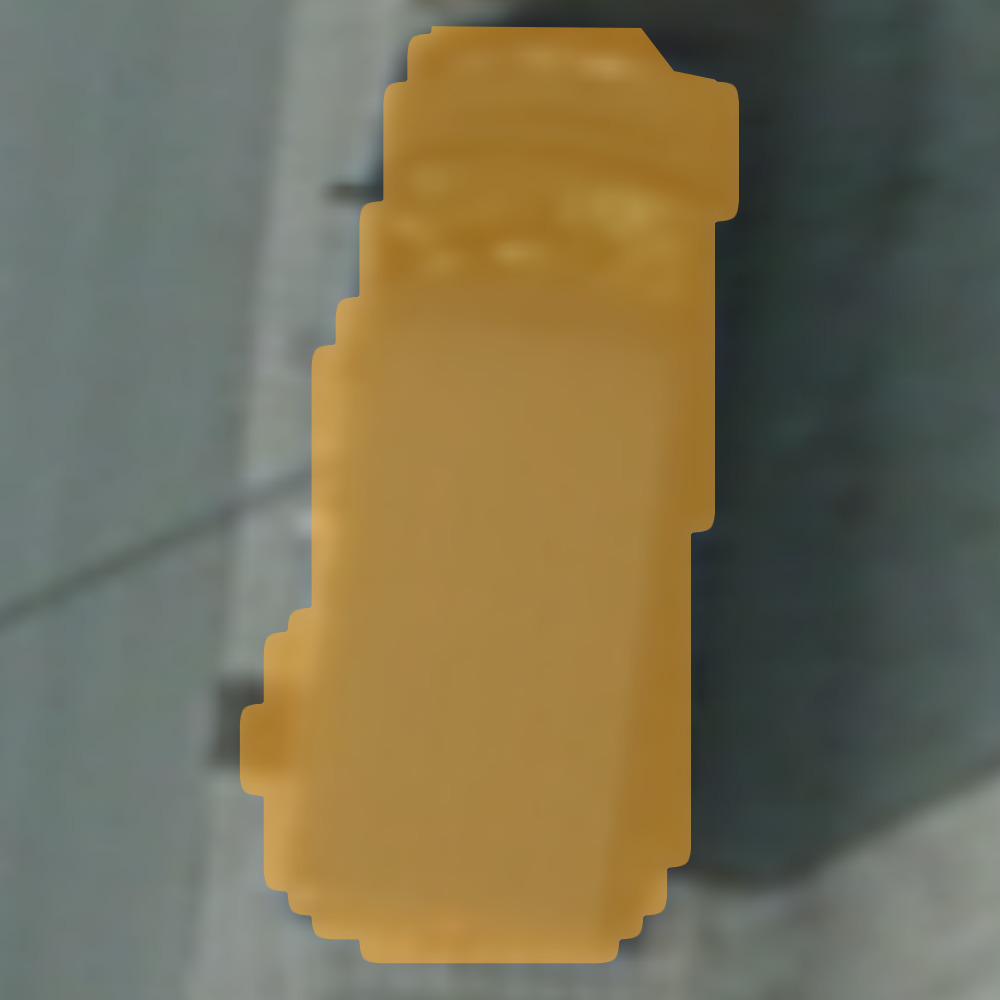
\includegraphics[width=\textwidth]{images/negative_example1}
     \caption{Van (camion prédit)}
   \end{subfigure}
  \begin{subfigure}{0.24\textwidth}
    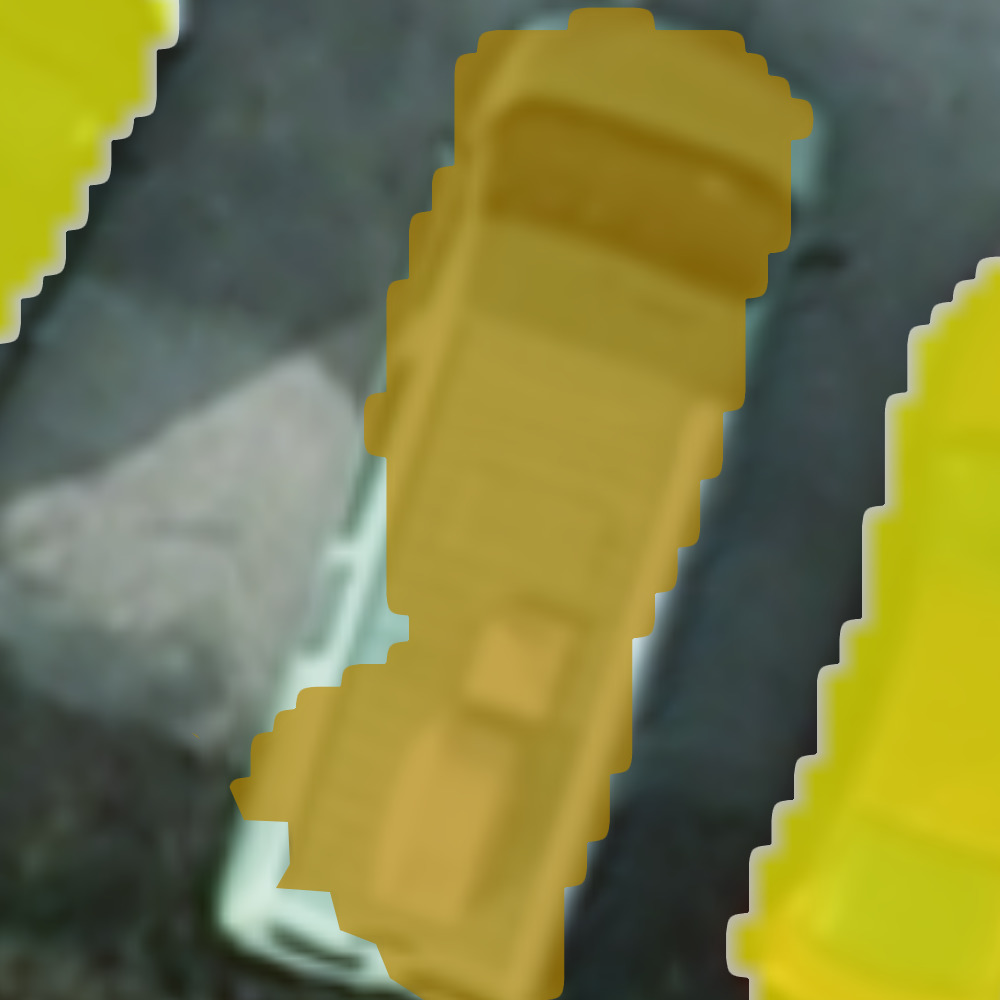
\includegraphics[width=\textwidth]{images/negative_example2}
    \caption{Van (camion prédit)}
  \end{subfigure}
  \begin{subfigure}{0.24\textwidth}
    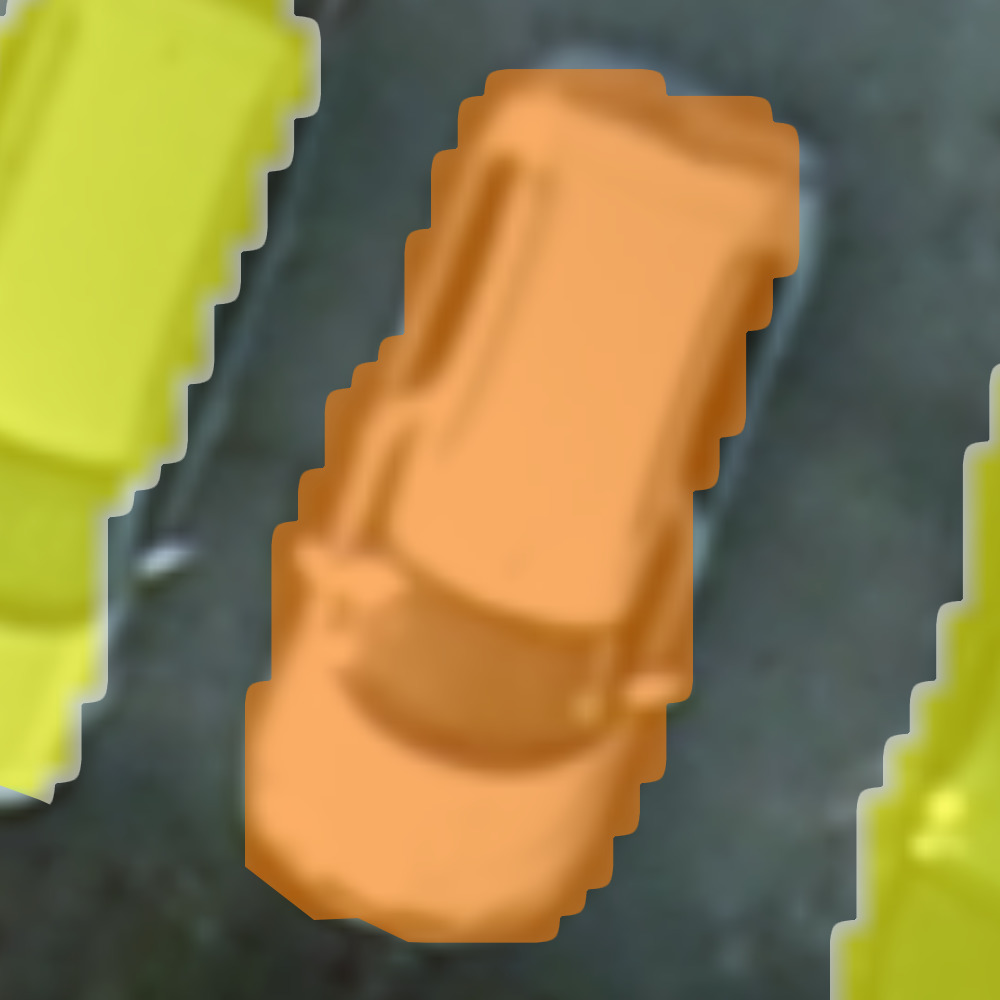
\includegraphics[width=\textwidth]{images/negative_example3}
    \caption{Voiture (van prédit)}
  \end{subfigure}
  \begin{subfigure}{0.24\textwidth}
    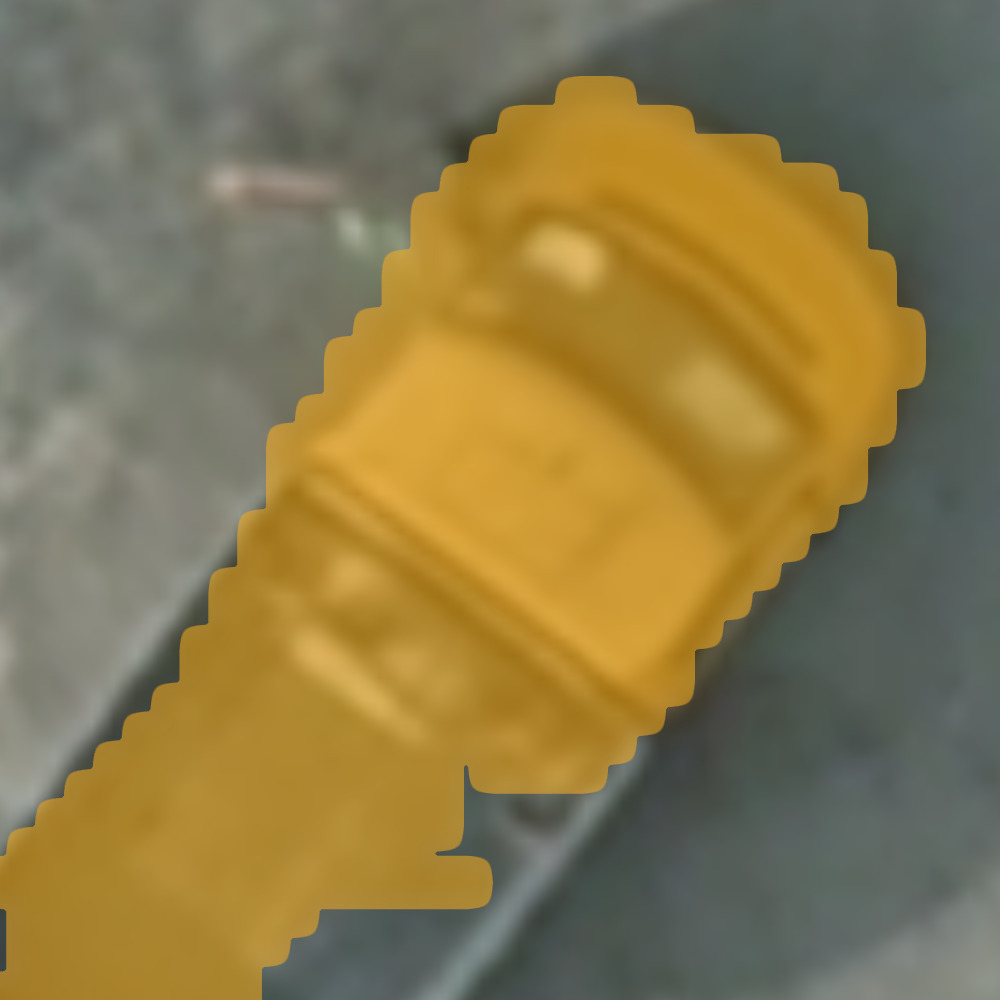
\includegraphics[width=\textwidth]{images/negative_example4}
    \caption{Pick-up (van prédit)}
  \end{subfigure}
  \caption{Segmentations réussies mais mauvaises classifications sur Potsdam.}
  \label{fig:negative_examples}
\end{figure}
\unskip
\begin{figure}[t]
\centering
  \begin{subfigure}{0.24\textwidth}
    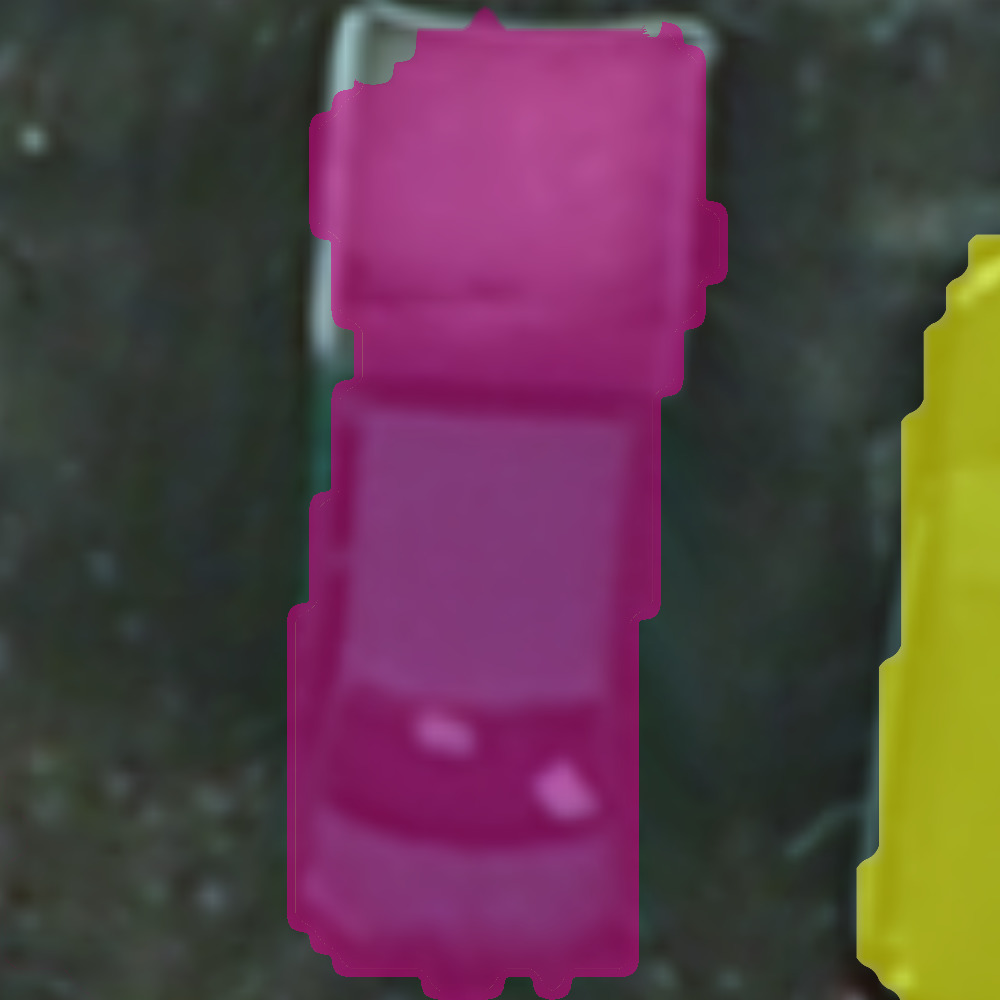
\includegraphics[width=\textwidth]{images/positive_example1}
    \caption{Pick-up}
  \end{subfigure}
%   \begin{subfigure}{0.24\textwidth}
%     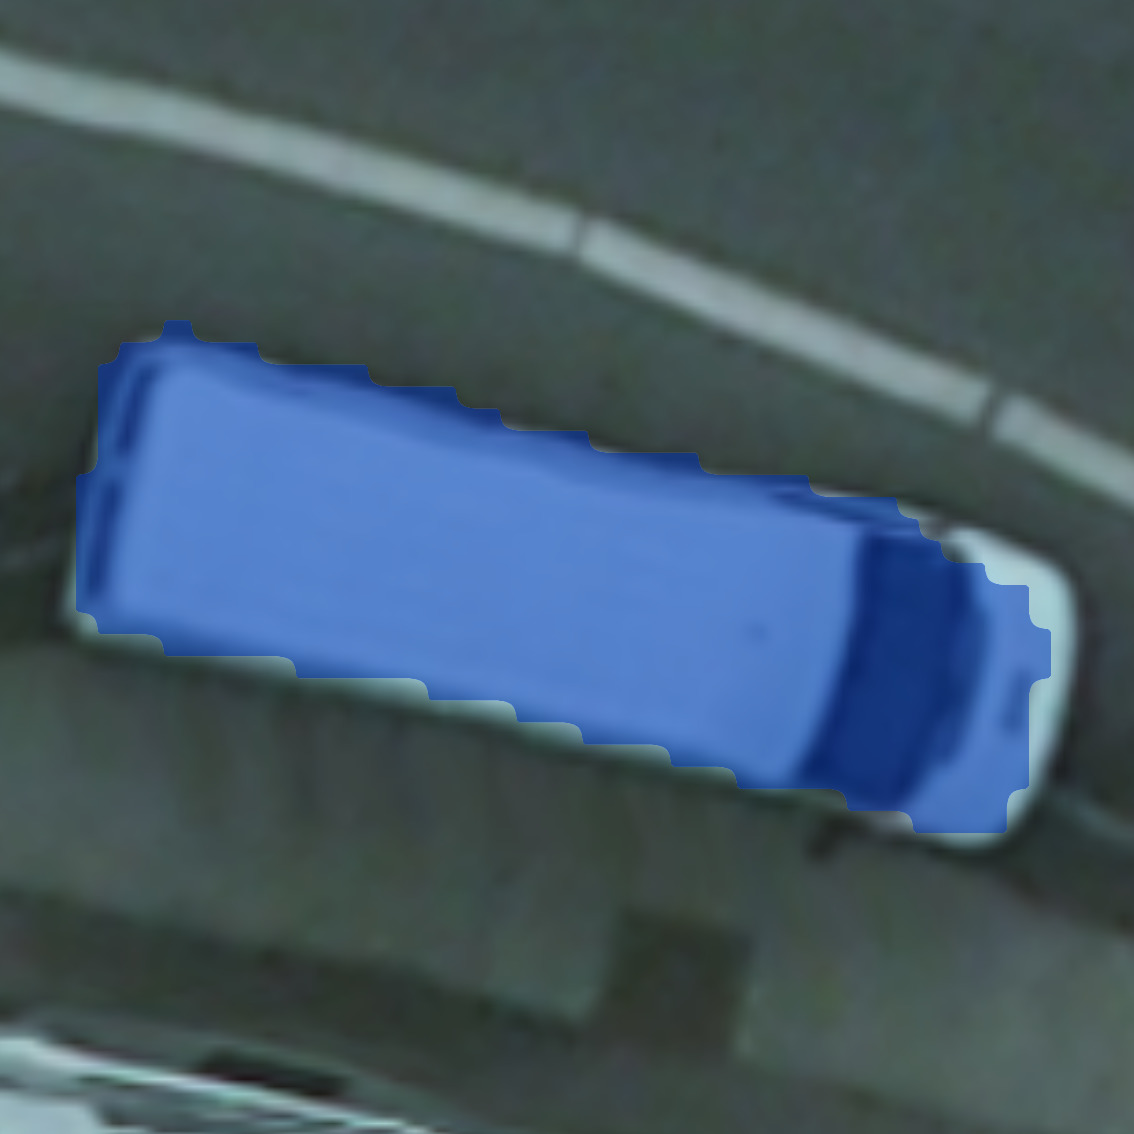
\includegraphics[width=\textwidth]{images/positive_example2}
%     \caption{Van}
%   \end{subfigure}
  \begin{subfigure}{0.24\textwidth}
    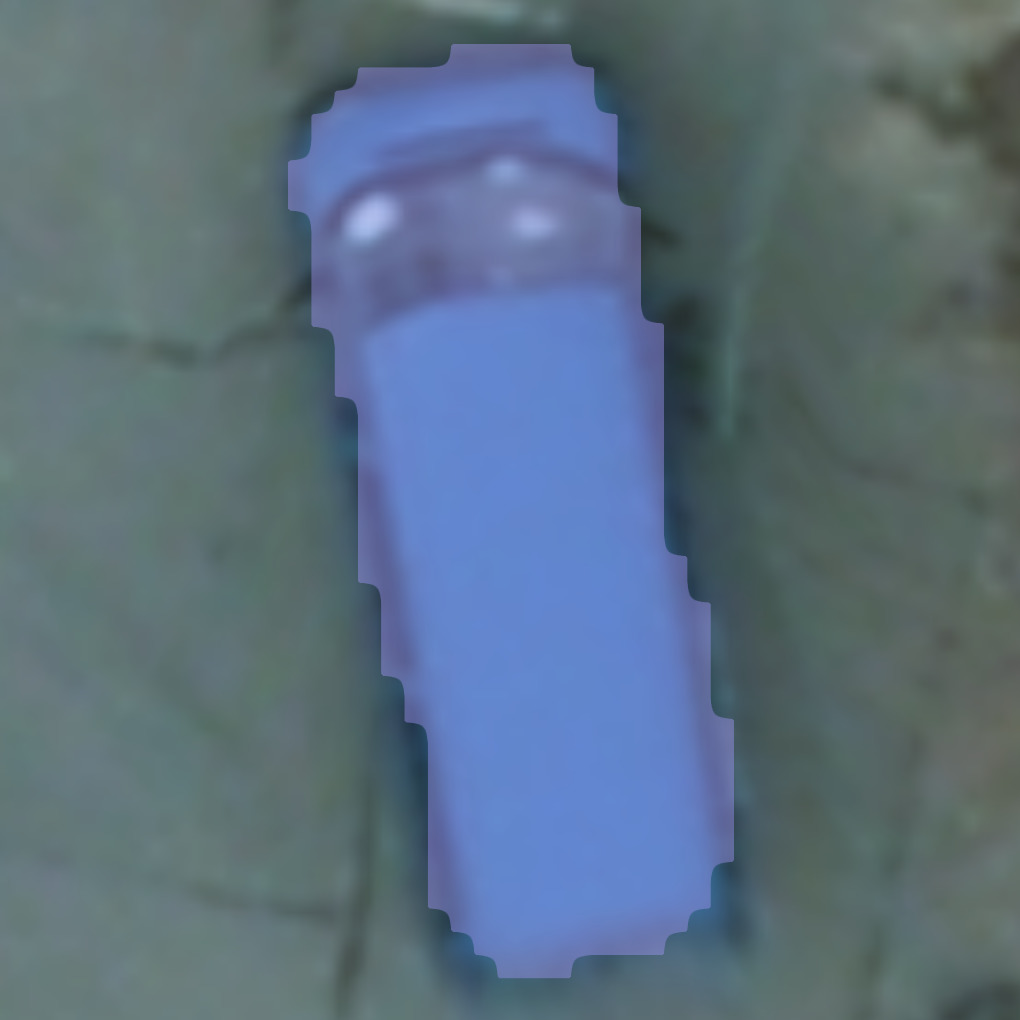
\includegraphics[width=\textwidth]{images/positive_example3}
    \caption{Van}
  \end{subfigure}
  \begin{subfigure}{0.24\textwidth}
    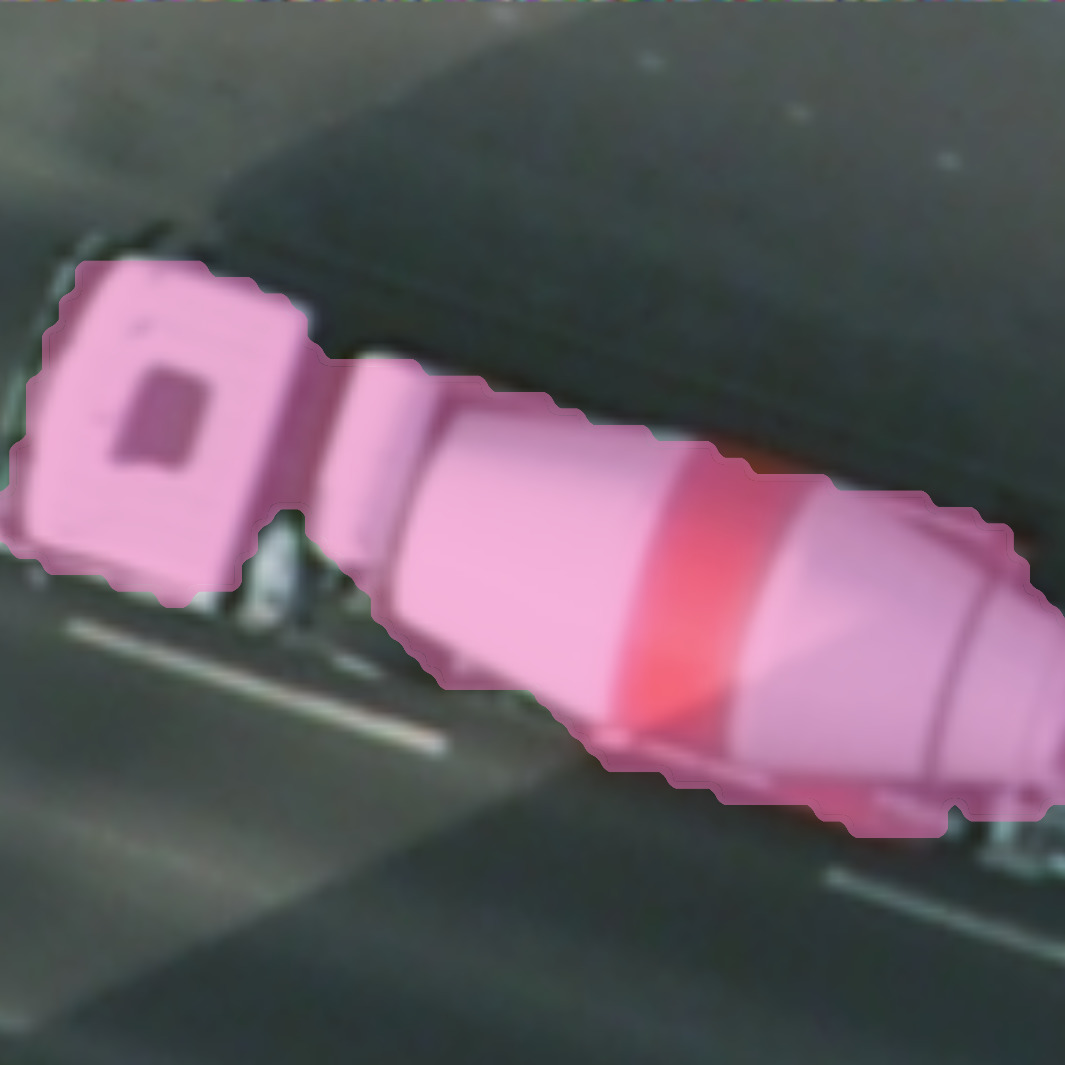
\includegraphics[width=\textwidth]{images/positive_example4}
    \caption{Camion}
  \end{subfigure}
  \begin{subfigure}{0.24\textwidth}
    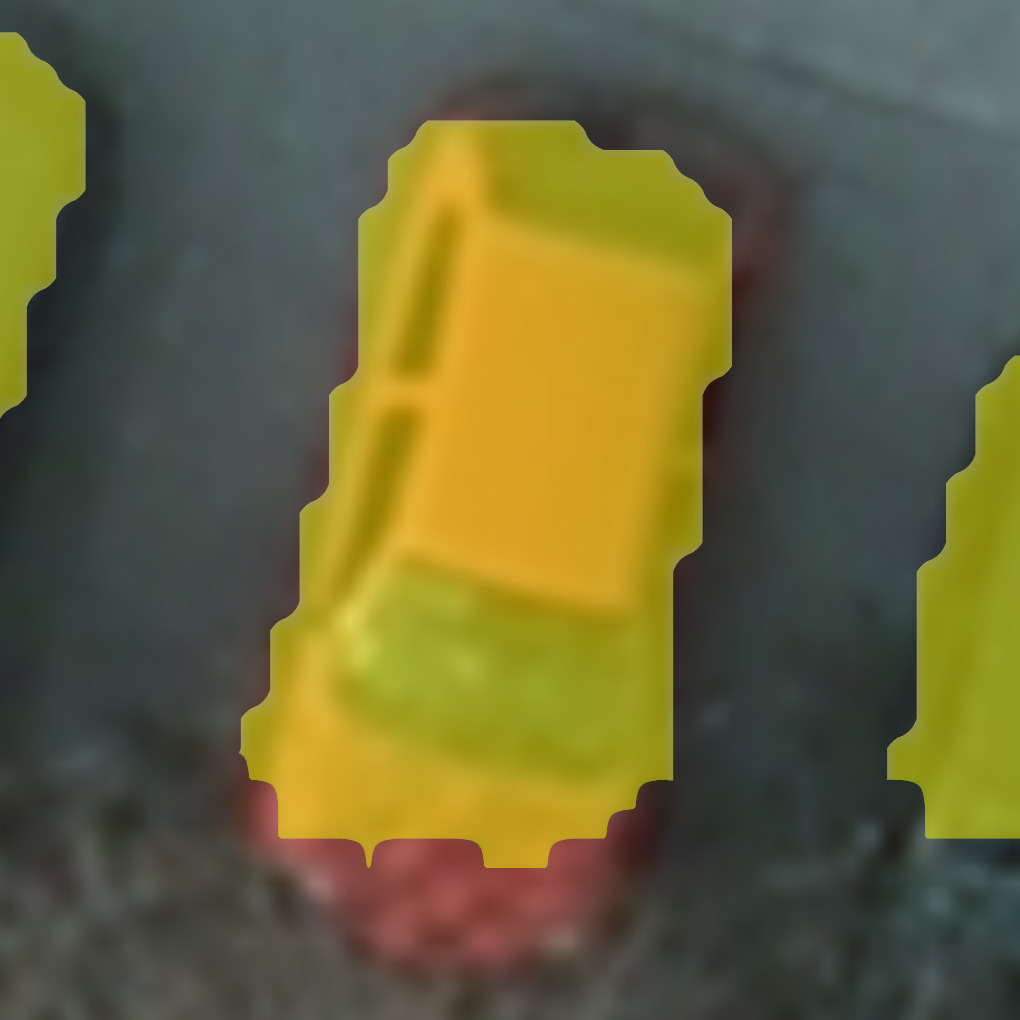
\includegraphics[width=\textwidth]{images/positive_example5}
    \caption{Voiture}
  \end{subfigure}

%   \begin{subfigure}{0.24\textwidth}
%     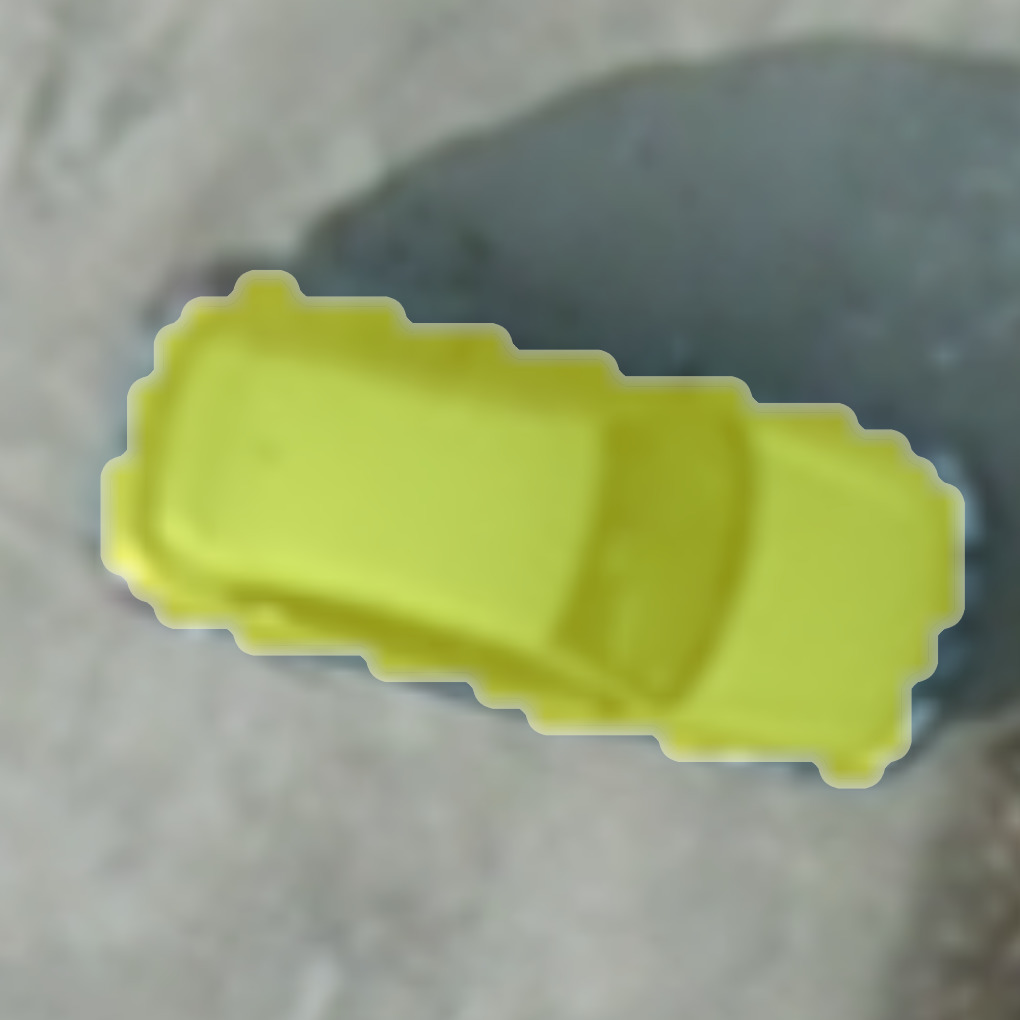
\includegraphics[width=\textwidth]{images/positive_example6}
%     \caption{Car}
%   \end{subfigure}
  \caption{Segmentations et classifications réussies sur Potsdam.}
  \label{fig:positive_examples}
\end{figure}

À ce stade, nous disposons d'un détecteur de véhicules efficace pour Potsdam et Christchurch et d'un classifieur entraîné sur \gls{VEDAI}. Le~\Cref{table:results_classif} détaille donc les résultats de classification du \gls{CNN} entraîné sur \gls{VEDAI} et appliqué aux véhicules de Potsdam et Christchurch. Les résultats sont agrégés par validation croisée sur les mêmes sous-divisions des jeux de données que pour les résultats en segmentation sémantique. Les voitures étant majoritaires dans les jeux de données considérés, nous indiquons également les résultats qui seraient obtenus par une heuristique de référence correspondant à un classifieur renvoyant systématiquement ``voiture''. Ce classifieur constant serait correct 94\% du temps, mais serait incapable de prédire autre chose qu'une voiture. L'exactitude globale du modèle serait donc excellente mais son exactitude moyenne catastrophique. Les \gls{CNN} parviennent quant à eux à prédire correctement plusieurs types de véhicules, augmentant significativement l'exactitude moyenne tout en maintenant une exactitude globale compétitive. Des exemples qualitatifs de bonnes segmentations mais mauvaises classifications et de bonnes segmentations et classifications sont illustrés dans les~\cref{fig:negative_examples,fig:positive_examples}.

\begin{table}[t]
\centering
  \caption{Résultats de classification de véhicules sur les vérité terrain augmentées de Potsdam et Christchurch}
  \label{table:results_classif}
  \begin{tabular}{cccccccc}
  \toprule
  \textbf{Jeu de données} & \textbf{Classifieur} & \textbf{Voiture} & \textbf{Van} & \textbf{Camion} & \textbf{Pick-up} & \textbf{OA} & \textbf{AA}\\
  \midrule
  %\multirow{3}{*}{Potsdam} & AlexNet & 81\% & 42\% & \textbf{50\%} & \textbf{50\%} & 75\% & 56\%\\
  %& VGG & 83\% & 55\% & \textbf{50\%} & 33\% & 77\% & 55\%\\
  %& AlexNet+R & \textbf{99\%} & \textbf{66\%} & 25\% & 0\% & \textbf{83\%} & 48\%\\
  \multirow{3}{*}{Potsdam} & Cars only & 100\% & 0\% & 0\% & 0\% & 94\% & 25\%\\
  & AlexNet & \textbf{98\%} & \textbf{66\%} & 67\% & 0\% & \textbf{95\%} & 58\%\\
  & VGG-16 & 92\% & 66\% & \textbf{75\%} & \textbf{33\%} & 89\% & \textbf{67\%}\\
  \midrule
  \multirow{3}{*}{Christchurch} & Cars only & 100\% & 0\% & 0\% & 0\% & 94\% & 25\%\\
  & AlexNet & 94\% & 40\% & \textbf{67\%} & \textbf{89\%} & 93\% & 73\%\\
  & VGG-16 & \textbf{97\%} & \textbf{80\%} & \textbf{67\%} & 78\% & \textbf{96\%} & \textbf{80\%}\\
  \bottomrule
  \end{tabular}
\end{table}

L'exactitude moyenne est plus basse sur Potsdam que sur \gls{VEDAI} compte-tenu du fort déséquilibre entre classes et la sensibilité numérique des résultats. En effet, chaque sous-division entraînement/test de la validation croisée contient environ 15 exemples de camions et de pick-ups. Cependant, le modèle est entraîné sur \gls{VEDAI}, dont la répartition entre classes n'est pas autant déséquilibrée. Par conséquent, le modèle possède un biais qui ne se transfère pas à Potsdam. En outre, les capteurs utilisés pour \gls{VEDAI}, Potsdam et Christchurch sont différents, tout comme les environnements considérés (urbain pour Potsdam et Christchurch, rural pour \gls{VEDAI}).

Les variations dues aux capteurs ont été corrigées en renormalisant la colorimétrie des images de Potsdam et Christchurch. Pour cela, nous estimons les moments statistiques des pixels sur \gls{VEDAI} et nous les appliquons à Potsdam et Christchurch:
\begin{equation}
X_{transformed} = \frac{X - m_{test~set}}{\sigma_{test~set}} \times \sigma_{train~set} + m_{train~set},
\end{equation}
avec $m$ la valeur du pixel moyen dans le jeu de données, $\sigma$ l'écart-type et $X$ l'image à transformer. Cette opération est appliquée sur chaque canal.

Toutefois, les différences d'apparence de l'environnement et surtout des types des véhicules diminuent tout de même les performances. Notamment, les voitures, camions et pick-ups sur Christchurch sont plus proches des marques américaines présentes dans \gls{VEDAI} que les véhicules de construction européenne présents dans Potsdam. Ces variations environnementales et d'apparence des objets peuvent faire sortir le classifieur de sa plage de fonctionnement.

Une régularisation adéquate ou un entraînement sur un jeu de données de véhicules plus varié pourrait permettre de limiter ces effets négatifs. De manière générale, ce type de transfert de connaissances est lié au problème d'adaptation de domaine non-supervisée~\cite{tuia_domain_2016,courty_optimal_2016}, qui est un sujet de recherche important en télédétection.

Finalement, nous avons donc montré qu'il était possible de récupérer \emph{a posteriori} la structure des objets segmentées par un \gls{FCN} directement depuis la classification pixel à pixel. Notamment, la méthode \emph{segment-before-detect} permet non seulement de détecter les véhicules dans des images aériennes, mais également d'identifier précisément leur forme et leur type. En particulier, cette méthode s'applique y compris dans le cas d'annotations imprécises, comme les boîtes englobantes de NZAM/ONERA Christchurch.
Toutefois, l'extraction des instances d'objet nécessite de faire appel à un processus \emph{ad hoc} permettant de regrouper les pixels appartenant à un même objet. Comme nous l'avons vu jusqu'ici, les modèles entièrement convolutifs sont optimisés pour minimiser une fonction de coût de classification pixel à pixel. Une telle fonction de coût ne permet pas de modéliser efficacement les dépendances spatiales pouvant exister entre les pixels, notamment leur appartenance à un même objet. Il paraît donc pertinent d'étudier comment rendre compte de ces relations spatiales dans l'optimisation des réseaux.

\section{Segmentation sémantique par régression des cartes de distances}

\subsection{Annotations sémantiques et cartes de distances}

Comme nous l'avons vu dans la section précédente, il est possible de reconstruire \emph{a posteriori} la structure des objets dans les cartes sémantiques prédites par un \gls{FCN}. Toutefois, la littérature relaie régulièrement des problèmes de frontières inter-classes imprécises ou de segmentations bruitées, nécessitant de faire appel à des régularisations a posteriori pour lisser les segmentations~\cite{zheng_conditional_2015,l._c._chen_deeplab_2018} ou à post-traitements \emph{ad hoc} comme la méthode \emph{segment-before-detect}.

La communauté s'est ainsi penchée sur différents post-traitements pour améliorer la netteté des contours et contraindre les segmentations à respecter la même topologie que la vérité terrain. Bien souvent, il s'agit de modèles graphiques ajoutés en fin de réseau~\cite{z._liu_deep_2017} ou faisant appel à des connaissances a priori~\cite{le_reformulating_2017,bertasius_semantic_2016}. La segmentation d'instance en particulier s'intéresse à combiner des approches de localisation géométrique avec des approches de sémantisation~\cite{he_mask_2017,dai_instance-aware_2015}.

Nous présentons ici une approche directe consistant en une régularisation implicite intégrée dans la représentation de la vérité terrain. En effet, nous proposons d'utiliser les cartes de distance issues des masques de segmentation comme tâche auxiliaire. Les cartes de distance indiquent non seulement l'appartenance d'un pixel à une classe donnée, mais également sa proximité spatiale vis-à-vis des autres classes d'intérêt et contient donc une information plus riche concernant la structure spatiale des données. Cette approche s'inscrit dans la veine de travaux sur l'utilisation de primitives géométriques pour régulariser la segmentation sémantique, comme la prédiction de l'orientation des objets~\cite{uhrig_pixel-level_2016} ou de la position de leur centre de masse~\cite{hayder_boundary-aware_2017}

De fait, en modifiant de façon minimale des réseaux de segmentation existants, nous parvenons à obtenir des segmentation plus régulières sans post-traitement ou connaissance a priori.

Nous validons notre méthode sur plusieurs architectures de réseaux convolutifs profonds et sur plusieurs applications en compréhension de scène urbaine, en segmentation d'images 2,5D et en observation de la Terre.

\subsubsection{Régularisation par régression des cartes de distances}
\begin{figure}[!t]
    \begin{subfigure}{0.33\textwidth}
    	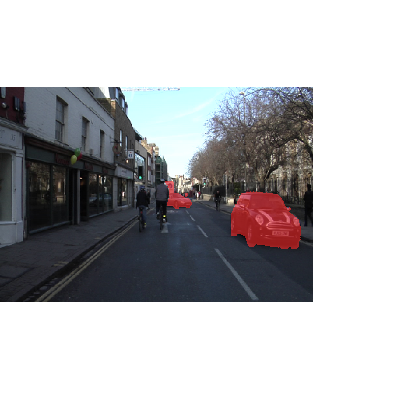
\includegraphics[width=\textwidth]{maskcars_colorbar}
        \caption{Masque binaire.}
    \end{subfigure}
    \begin{subfigure}{0.33\textwidth}
    	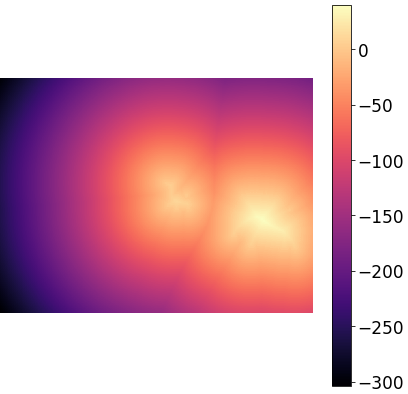
\includegraphics[width=\textwidth]{distcars_colorbar}
        \caption{\Glsdesc{CDS}}
    \end{subfigure}
    \begin{subfigure}{0.33\textwidth}
    	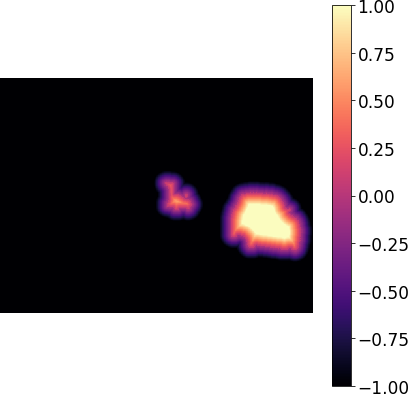
\includegraphics[width=\textwidth]{distcars_normalized_colorbar}
        \caption{\glssymbol{CDS} tronquée et normalisée.}
    \end{subfigure}

	\begin{subfigure}{0.33\textwidth}
    	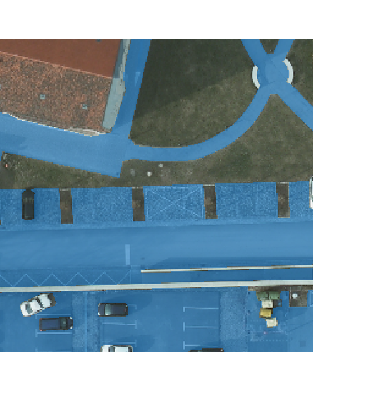
\includegraphics[width=\textwidth]{potsdam_maskroad_zoom}
        \caption{Masque binaire.}
    \end{subfigure}
    \begin{subfigure}{0.33\textwidth}
    	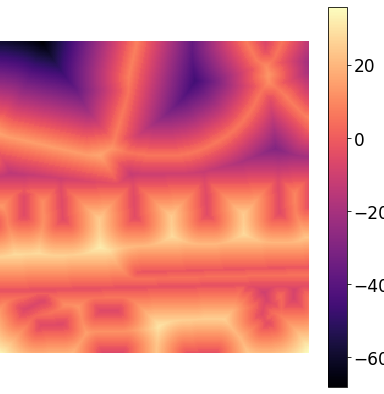
\includegraphics[width=\textwidth]{potsdam_distroad_zoom_colorbar}
        \caption{\Glsdesc{CDS}}
    \end{subfigure}
    \begin{subfigure}{0.33\textwidth}
    	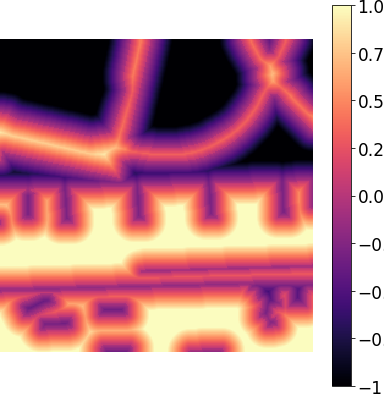
\includegraphics[width=\textwidth]{potsdam_distroadnorm_zoom_colorbar}
        \caption{\glssymbol{CDS} tronquée et normalisée.}
    \end{subfigure}
    \caption{Différentes représentations de segments annotés.}
    \label{fig:representations}
\end{figure}

Ce travail s'intéresse à l'utilisation des \glspl{CDS} pour régulariser des réseaux de segmentation sémantique. Le passage en carte de distances transforme un masque binaire en une représentation équivalente mais à valeurs continues. En l'occurence, nous travaillons avec des cartes de distances signées tronquées puis renormalisées dans $[-1,1]$. Ces représentations des annotations sont illustrées dans la~\cref{fig:representations}. Nous émettons l'hypothèse que cette représentation permet toutefois d'accéder plus directement à la structure spatiale des données, notamment car elle contient pour un pixel sa distance spatiale relative à toutes les classes d'intérêt. Cette représentation est donc plus riche en quantité d'information que les masques binaires utilisés pour la classification. Nous montrons que l'utilisation de la régression des \glspl{CDS} en tâche auxiliaire d'un réseau de segmentation sémantique a des résultats bénéfiques sur la segmentation finale.

\subsubsection{Transformée de distances}

La transformée de distances (ou carte de distances) d'une image binaire assigne à chaque pixel du maillage sa distance au point positif du masque le plus proche. La distance peut être calculée en utilisant différentes métriques, comme la distance Manhattan ou la distance Euclidienne. Pour les éléments appartenant au masque positif (premier-plan), la distance est conventionnellement 0. Par exemple, la transformée $\mathcal{D}$ de distances euclidienne transforme une image $I$ de dimensions $M\times N$ de masque positif $I^+$ en une carte de distance $\mathcal{D}(I)$ obtenue par:
\begin{equation}
  \forall i,j \in M\times N, ~~~\mathcal{D}(I)[i,j] = \min_{I_{i',j'} \in I^+} (\parallel I[i,j] - I[i',j'] \parallel)~~~.
\end{equation}

En pratique, nous utilisons la transformée de distances signée~\cite{q._z._ye_signed_1988}, qui associe à chaque pixel du premier plan sa distance positive au pixel de l'arrière-plan le plus proche et à chaque pixel de l'arrière-plan l'opposé de sa distance au pixel du premier plan le plus proche. Formellement, il s'agit de la transformée $\mathcal{D}_s$ qui associe à $I$ son image:
\begin{equation}
\forall i,j \in M\times N,~~~\mathcal{D}_s(I)[i,j] =
\begin{cases}
+ \min_{I_{i',j'} \in I^-} (\parallel I[i,j] - I[i',j'] \parallel), & \text{si}~I[i,j] \in I^+,\\
- \min_{I_{i',j'} \in I^+} (\parallel I[i,j] - I[i',j'] \parallel), & \text{si}~I[i,j] \notin I^-.\\
\end{cases}
\end{equation}

Les annotations de segmentation sémantique correspondent en pratique à un masque binaire par classe. Il est donc possible de convertir ces annotations en leur contrepartie sous forme de \gls{CDS}. Il est important de souligner qu'aucune information n'est perdue dans ce procédé, les masques binaires pouvant être retrouvées par simple seuillage des \glspl{CDS}. Nous appliquons donc la transformée de distances signée aux annotations en utilisant l'algorithme exact en temps linéaire de~\citet{maurer_linear_2003}.

Pour limiter des effets indésirables lorsque les pixels sont très éloignés de certains objets, de sorte que lesdits objets ne sont plus visibles dans le champ réceptif du réseau, nous ajoutons une saturation aux distances calculées. En particulier, nous normalisons la \gls{CDS} dans $[-1, 1]$ en lui appliquant une transformation $\operatorname{hardtanh}$. Ces différentes représentations sont illustrées dans la~\cref{fig:representations}.

\begin{figure*}[!t]
	\centering
	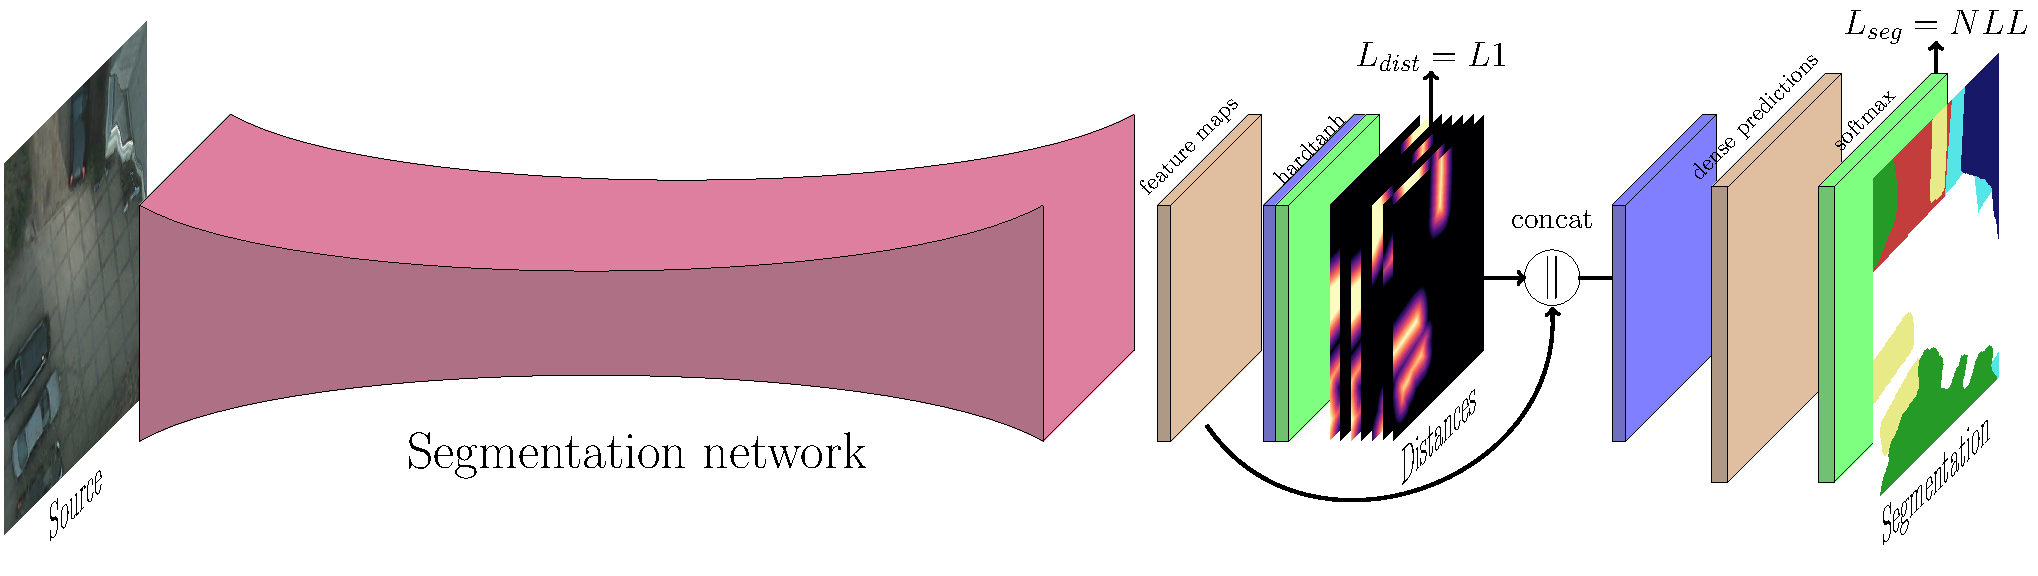
\includegraphics[width=0.9\textwidth]{multitask_distances}
    \caption{Apprentissage multi-tâche (classification pixel à pixel et régression des cartes de distances). Les couches convolutives sont en {\color{blue}bleu}, les activations non-linéaires en {\color{green!50!black}vert} et les cartes d'activation en {\color{brown}marron}.}
    \label{fig:distance_framework}
\end{figure*}

\subsection{Apprentissage multi-tâche}

%Signed distance transform maps are continuous representations of the labels. We can train a deep network to approximate these maps using a regression loss.

La régression directe des \glspl{CDS} ne permet pas d'obtenir de meilleurs résultats de segmentation que la classification dense pixel à pixel usuelle. De fait, nous proposons donc d'utiliser une stratégie d'apprentissage multi-tâche dans laquelle le réseau est optimisé à la fois sur la classification des pixels et sur la régression des \glspl{CDS}.
%However, preliminary experiments show that training only for regression does not bring any improvement compared to traditional classification and even degrades the results.
%sl% penses-tu qu'il faudrait donner des résultats ici ou juste le dire?
%Therefore, we suggest to use a multi-task strategy, in which the network learns both the classification on the usual one-hot labels and the regression on the SDT.

En particulier, nous modifions l'architecture du réseau pour, dans un premier temps, effectuer la régression des \glspl{CDS}; puis nous ajoutons une couche convolutive additionnelle pour fusionner les activations de la dernière couche avec les \glspl{CDS} prédites afin de réaliser la classification finale. Le réseau est ainsi entraîné en multi-tâche, la régression des \glspl{CDS} étant utilisée comme tâche intermédiaire avant la classification.
%More precisely, we alter the network to first predict the SDT and we then use an additional convolutional layer to fuse the last layer features and the inferred SDT to perform the final classification. In this way, the network is trained in a cascaded multi-task fashion, where the distance transform regression is used as a proxy, i.e. an intermediate task, before classification.

L'altération du réseau se résume comme suit. La dernière couche, habituellement suivie d'un \textit{softmax} est ici utilisée comme couche de régression des \glspl{CDS}. Les distances étant normalisées entre $-1$ et $1$, la fonction $hardtanh$ est utilisée comme activation non-linéaire. Puis nous concaténons les activations de la couche précédente aux \glspl{CDS} ainsi prédites pour alimenter une couche convolutive additionnelle suivie d'un \textit{softmax}. L'architecture complète est illustrée dans la~\cref{fig:distance_framework}.
%Therefore, the network modification can be summarized as follows. Instead of using the last layer and feeding it into a softmax, we now use the last layer as a distance prediction. As distances are normalized between -1 and 1, these distances pass through a $hardtanh$ non-linearity. Then, we concatenate the previous layer features maps and the distance predictions to feed both into a convolutional and a softmax layer. The complete architecture is illustrated in~\cref{fig:distance_framework}.

Par souci d'équité dans nos expériences, les modèles de référence présentés dans la~\cref{sec:experiments} utilisent également une couche de convolution additionnelle afin que tous les modèles équivalents possèdent le même nombre de paramètres optimisables.
%For a fair comparison, the classification baselines considered in~\cref{sec:experiments} use the same additional convolutional layer, so that both models have the same number of parameters.

Les fonctions de coût utilisées dans ces travaux sont la log-vraisemblance négative (NLL) pour la classification et la distance L1 pour la régression.
%In this work, we keep the traditional cross-entropy loss for classification, in the form of the negative log-likelihood (NLL). As our regression results are constrained in $[-1;1]$, we use the L1 loss to preserve relative errors.

En notant respectivement $Z_{seg}, Z_{dist}, Y_{seg}, Y_{dist}$ la classification après \textit{softmax}, la carte de distances prédite, les annotations de vérité terrain et la carte de distances réelle, la fonction de coût à minimiser est:
%Assuming that $Z_{seg}, Z_{dist}, Y_{seg}, Y_{dist}$ respectively denote the output of the segmentation softmax, the regressed distance, the ground truth segmentation labels and the ground truth distances, the final loss to be minimized is:
\begin{equation}
L = NLL(Z_{seg}, Y_{seg}) + \lambda L1(Z_{dist}, Y_{dist})
\end{equation}
%where $\lambda$ is an hyper-parameter that controls the strength of the regularization.
où $\lambda$ est un hyperparamètre contrôlant l'amplitude de la régularisation.

\subsection{Validation expérimentale}

Afin de pouvoir mesurer l'effet de la régression des cartes de distance, nous entraînons des réseaux avec l'architecture SegNet~\cite{badrinarayanan_segnet_2017} ou PSPNet~\cite{zhao_pyramid_2017} de référence, soit en régression pure, soit en classification pure.
%We first obtain baseline results on various datasets using SegNet or PSPNet for semantic segmentation, either using the cross entropy for label classification or the L1 loss for distance regression. However, note that our method is not architecture-dependent. It consists in a straightforward modification of the end of the network that would fit any architecture designed for semantic segmentation.

L'architecture encodeur-décodeur SegNet~\cite{badrinarayanan_segnet_2017} a déjà été présentée au \cref{chap:cartographie}. PSPNet~\cite{zhao_pyramid_2017} est une architecture entièrement convolutive ayant établi un nouvel état de l'art sur plusieurs jeux de données de segmentation sémantique~\cite{cordts_cityscapes_2016,everingham_pascal_2014}. Elle dérive du modèle ResNet~\cite{he_deep_2016} et utilise un module de concaténation en pyramide d'activations pour prendre en compte plusieurs niveaux de contexte spatial. Dans notre cas, nous utilisons une version réduite de PSPNet conçue sur l'architecture ResNet-101. ResNet-101 produit des cartes d'activation à résolution $1{:}32$ qui sont suréchantillonnées par déconvolution.
%PSPNet~\cite{zhao_pyramid_2017} is a recent model for semantic segmentation that achieved new state-of-the-art results on several datasets~\cite{cordts_cityscapes_2016,everingham_pascal_2014}. It is based on the popular ResNet~\cite{he_deep_2016} model and uses a pyramidal module at the end to incorporate multi-scale contextual cues in the learning process. In our case, we use a smaller albeit efficient version of PSPNet based on ResNet-50~\cite{he_deep_2016}. ResNet-50 encodes the input into feature maps at 1:32 resolution, which are then upsampled using transposed convolutions.

\subsubsection{Jeux de données}

\begin{table*}[!t]
  \setlength\tabcolsep{3pt}
  \caption{Résultats de validation croisée sur les jeux de données ISPRS. Les valeurs indiquées représentent le taux global de bonne classification et le score F1 pour chaque classe.}
  \label{tab:isprs_results}
\begin{tabularx}{\textwidth}{c Y Y Y Y Y Y Y}
\toprule
Méthode & Ville & \% classification & Routes & Bâtiments & Vég. basse & Arbres & Véhicules\\
\midrule
% Regression (lambda = +inf) OA : 89.49 +- 0.86 F1 : 91.03 +- 1.35 F1 : 95.60 +- 0.26 F1 : 81.23 +- 2.76 F1 : 88.31 +- 1.99 F1 : 0.00 +- 0.00
SegNet* (régression) & \multirow{3}{*}{Vaihingen} & 89.49 & 91.03 & 95.60 & 81.23 & 88.31 & 0.00\\
% Classif (lambda = 0) : OA : 90.00 +- 1.17 F1 : 91.98 +- 1.62 F1 : 95.53 +- 0.20 F1 : 80.91 +- 2.62 F1 : 88.07 +- 2.33 F1 : 87.94 +- 1.76
SegNet* (classification) & & 90.00 & 91.98 & 95.53 & 80.91 & 88.07 & 87.94\\
% Multi-task (lambda = 2) : OA : 90.43 +- 1.00 F1 : 92.46 +- 1.41 F1 : 95.99 +- 0.24 F1 : 81.30 +- 2.96 F1 : 88.34 +- 2.09 F1 : 88.16 +- 1.24
SegNet* (multi-tâche) & & \textbf{90.43} & \textbf{92.46} & \textbf{95.99} & \textbf{81.30} & \textbf{88.34} & \textbf{88.16}\\
\midrule
%SegNet (regression) & \multirow{3}{*}{Potsdam} & ? & ? & ? & ? & ? & ?\\
% Classif (lambda = 0) OA : 91.85 +- 1.19 F1 : 94.12 +- 0.37 F1 : 96.09 +- 1.02 F1 : 88.48 +- 0.56 F1 : 85.44 +- 1.93 F1 : 96.62 +- 0.30
SegNet* (classification) & \multirow{2}{*}{Potsdam} & 91.85 & 94.12 & 96.09 & 88.48 & 85.44 & 96.62\\
% Multi-task (lambda = 2) : OA : 92.22 +- 1.15 F1 : 94.33 +- 0.45 F1 : 96.52 +- 1.03 F1 : 88.55 +- 0.62 F1 : 86.55 +- 1.28 F1 : 96.79 +- 0.37
SegNet* (multi-tâche) & & \textbf{92.22} & \textbf{94.33} & \textbf{96.52} & \textbf{88.55} & \textbf{86.55} & \textbf{96.79}\\
\bottomrule
\end{tabularx}
\end{table*}

Nous validons notre approche sur plusieurs jeux de données afin de démontrer sa capacité à généraliser dans des contextes de segmentation mono et multi-classe sur plusieurs types d'images.
%We validate our method on several datasets in order to show its generalization capacity on multi and mono-class segmentation of both ground and aerial images.

\paragraph{ISPRS 2D Semantic Labeling}

Le jeu de données ISPRS 2D Semantic Labeling~\cite{rottensteiner_isprs_2012} est constitué des scènes Potsdam et Vaihingen, déjà présentées aux chapitres précédents et détaillés dans l'\cref{annexe:isprs}. L'évaluation est réalisée par validation croisée en divisant les jeux de données en trois plis.

\paragraph{INRIA Aerial Image Labeling Benchmark}
Le jeu de données INRIA Aerial Image Labeling~\cite{maggiori_can_2017} contient 360 images RVB de taille $5000\times5000$px à une résolution de 30cm/px, couvrant 10 agglomérations de divers points du globe. La moitié des villes sont utilisées pour l'apprentissage et associées à des annotations publiques d'empreintes de bâtiments. Le reste du jeu de données est utilisé pour l'évaluation. Plus d'informations sont données dans l'\cref{annexe:inria}.

\paragraph{SUN RGB-D}
Le jeu de données SUN RGB-D~\cite{song_sun_2015} contient 10 335 images RVB accompagnées d'une carte de profondeur. Ces images ont été annotées sur 37 classes d'intérêt comportant le mobilier, les murs, le sol\dots Il vise principalement à évaluer les capacités d'interprétation d'images dans un cadre de navigation robotique en intérieur, avec des objets à moins de \SI{10}{\meter}. Plus d'informations sont données dans l'\cref{annexe:sun}.

%\paragraph{Data Fusion Contest 2015}
%The Data Fusion Contest 2015~\cite{campos-taberner_processing_2016} is comprised of 7 aerial RGB images of $10,\!000\times10,\!000$px with a spatial resolution of 5cm/px on the city of Zeebruges, Belgium. A dense set of annotations on 8 classes (6 from ISPRS dataset plus ``water'' and ``boat'') is given. Two images are reserved for testing, we use one image for validation and the rest for training.
%We extract $256\times256$ patches from the training tiles, augmented by vertical and horizontal symmetries. Inference is done by sliding a $256\times256$ window with a stride of 32px on the test tiles.

\paragraph{CamVid}
Le jeu de données CamVid~\cite{brostow_semantic_2009} comporte 701 images extraites de plusieurs vidéos filmées par une caméra embarquée dans une voiture, avec une résolution de $360\times480$px. Nous utilisons la même division du jeu de données que~\cite{badrinarayanan_segnet_2017}, c'est-à-dire 367 images d'apprentissage, 101 images de validation et 233 images de test. Les annotations recouvrent 11 classes d'intérêt telles que ``bâtiment'', ``piéton'', ``voiture'' ou encore ``trottoir''. Plus de détails sont donnés dans l'\cref{annexe:camvid}.

\subsubsection{Protocole expérimental}

Les architectures SegNet et PSPNet-101 sont entraînées et déployées de la façon suivante.

SegNet est entraîné pendant 50\,000 itérations sur des \emph{mini-batches} de 10 images. L'optimisation se fait par descente de gradient stochastique avec un taux d'apprentissage de 0,01, divisé par 10 après 25\,000 et 45\,000 itérations. Les poids de l'encodeur sont initialisés avec ceux de VGG-16~\cite{simonyan_very_2014} pré-entraîné sur ImageNet. Les poids du décodeur sont initialisés aléatoirement en utilisant la stratégie proposée dans~\cite{he_delving_2015}.
%SegNet is trained for 50 epochs with a batch size of 10. Optimization is done using Stochastic Gradient Descent (SGD) with a base learning rate of 0.01, divided by 10 after 25 and 45 epochs, and a weight decay set at 0.0005. Encoder weights are initialized from VGG-16~\cite{simonyan_very_2014} trained on ImageNet~\cite{deng_imagenet:_2009}, while decoder weights are initialized using the policy from~\cite{he_delving_2015}.
Pour le jeu de données multi-modal SUN RGB-D, nous utilisons le modèle FuseNet~\cite{hazirbas_fusenet_2016}, qui consiste en un SegNet à double entrée.
%For SUN RGB-D, in order to validate our method in a multi-modal setting, we use the FuseNet~\cite{hazirbas_fusenet_2016} architecture. This model consists in a dual-stream SegNet that learns a joint representation of both the color image and the depth map. We train it using SGD with a learning rate of 0.01 on resized $224\times224$ images.
Sur les images aériennes, nous augmentons le nombre d'échantillons d'apprentissage en extrayant des images de $256\times256$ ($384\times384$ pour le jeu de données INRIA Aerial Image) et en procédant aléatoirement à des symétries horizontales ou verticales. L'inférence est réalisée avec une fenêtre glissante de même dimension et un recouvrement de 75\%.
%On aerial images, we randomly extract $256\times256$ ($384\times384$ on the INRIA Labeling dataset), augmented with flipping and mirroring. Inference is done using a sliding window of the same shape with a 75\% overlap.

PSPNet est entraîné sur CamVid pendant 750\,000 itérations sur 10 images en parallèle par descente de gradient stochastique avec un taux d'apprentissage de 0,01, divisé par 10 après 500\,000 itérations. Nous extrayons aléatoirement des imagettes de $224\times224$ et nous appliquons aléatoirement une symétrie horizontale. Suivant le protocole de~\cite{jegou_one_2017}, nous raffinons l'apprentissage en entraînant pendant 200\,000 itérations sur les images à pleine résolution.
%We train a PSP-Net on CamVid for 750 epochs using SGD with a learning rate of 0.01, divided by 10 at epoch 500, a batch size of 10 and a weight decay set at 0.0005. We extract random $224\times224$ crops from the original images and we perform random mirroring to augment the data. We fine-tune on full scale images for 200 epochs, following the practice from~\cite{jegou_one_2017}.
Notre implémentation de PSPNet utilise les poids de ResNet-101~\cite{he_deep_2016} pré-entraînés sur ImageNet pour l'initialisation, et n'utilise pas la fonction de coût auxiliaire présentée dans~\cite{zhao_pyramid_2017}.
%Our implementation of PSPNet is based on ResNet-50 pre-trained on ImageNet and do not use the auxiliary classification loss for deep supervision~\cite{zhao_pyramid_2017}.

Finalement, nous compensons le déséquilibre des classes dans les jeux de données SUN RGB-D et CamVid en utilisant une pondération relativement à la fréquence médiane.
%Finally, we use median-frequency balancing to alleviate the class unbalance from SUN RGB-D and CamVid.

Toutes les expériences sont réalisées à l'aide de la bibliothèque PyTorch~\cite{noauthor_pytorch_2016}. les \glspl{CDS} sont calculées sur \glssymbol{CPU} à l'aide de la bibliothèque Scipy~\cite{jones_scipy_2001} et conservées en mémoire pour éviter les calculs redondants. Le calcul des \glspl{CDS} ralentit légèrement l'entraînement lors des premières itérations, afin leur mise en cache. Dans un cadre applicatif concret, une implémentation en ligne sur GPU~\cite{zampirolli_fast_2017} permettrait d'effectuer ces calculs en ligne rapidement sans nécessiter de surcoût mémoire.

\begin{figure}[t]
\begin{subfigure}{0.24\textwidth}
	\includegraphics[width=\textwidth]{images_vaihingen/top_mosaic_09cm_area32}
    \caption{Image IRRV}
\end{subfigure}
\begin{subfigure}{0.24\textwidth}
	\includegraphics[width=\textwidth]{images_vaihingen/top_mosaic_09cm_area32_gt_colors}
    \caption{Vérité terrain}
\end{subfigure}
\begin{subfigure}{0.24\textwidth}
	\includegraphics[width=\textwidth]{images_vaihingen/result_segnet_256_proxy_0_32_colors}
    \caption{SegNet (classification)}
\end{subfigure}
\begin{subfigure}{0.24\textwidth}
	\includegraphics[width=\textwidth]{images_vaihingen/result_segnet_256_proxy_2_32_colors}
    \caption{SegNet (multi-tâche)}
\end{subfigure}
\caption{Extrait des résultats de segmentation sur le jeu de données ISPRS Vaihingen.\\\isprslegende}
\label{fig:isprs_vaihingen}
\end{figure}

\begin{figure}[t]
\begin{subfigure}{0.24\textwidth}
	\includegraphics[width=\textwidth]{images_potsdam/top_potsdam_2_11_RGB}
    \caption{Image RVB}
\end{subfigure}
\hfill
\begin{subfigure}{0.24\textwidth}
	\includegraphics[width=\textwidth]{images_potsdam/top_potsdam_2_11_label_gt_colors}
    \caption{Vérité terrain}
\end{subfigure}
\hfill
\begin{subfigure}{0.24\textwidth}
	\includegraphics[width=\textwidth]{images_potsdam/result_segnet_potsdam_256_proxy_0_2_11_colors}
    \caption{SegNet (classification)}
\end{subfigure}
\hfill
\begin{subfigure}{0.24\textwidth}
	\includegraphics[width=\textwidth]{images_potsdam/result_segnet_potsdam_256_proxy_2_2_11_colors}
    \caption{SegNet (multi-tâche)}
\end{subfigure}
\caption{Extrait des résultats de segmentation sur le jeu de données ISPRS Potsdam.\\\isprslegende}
\label{fig:isprs_potsdam}
\end{figure}

\subsubsection{Résultats}

Dans les~\cref{tab:isprs_results,tab:inria_results,tab:sun_results,tab:camvid_results}, les modèles signalés par une étoile (``*'') sont ceux proposés dans le cadre cette étude et implémentés par nos soins. Les autres modèles sont des références de l'état de l'art.

\paragraph{ISPRS dataset}
Les résultats de validation croisée sur les jeux de données ISPRS Vaihingen et Potsdam sont détaillés dans le~\cref{tab:isprs_results}. Toutes les classes semblent bénéficier de la régression des cartes de distances. En particulier, les arbres sur Potsdam sont significativement mieux segmentés, la régression de la CDS contraignant le réseau à prendre en compte la convexité naturelle de l'objet en dépit de l'absence de feuilles. Deux exemples de segmentation sont présentés en~\cref{fig:isprs_vaihingen} et~\cref{fig:isprs_potsdam}, dans lesquelles on peut voir que les bâtiments bénéficient grandement de l'approche multi-tâche (apparence plus lisse et moins de bruit de classification). Nous avons également testé l'approche par régression seule sur le jeu de données ISPRS Vaihingen avec des résultats mitigés. En effet, la plupart des classes bénéficient de ce traitement mais le réseau devient alors incapable de segmenter les véhicules, provoquant dans l'ensemble une baisse du taux de bonne classification.
%The cross-validated results on the ISPRS Vaihingen and Potsdam datasets are reported in~\cref{tab:isprs_results}. All classes seem to benefit from the distance transform regression. On Potsdam, the class ``trees'' is significantly improved as the distance transform regression forces the network to better learn its closed shape, despite the absence of leaves that make the underlying ground visible from the air. Two example tiles are shown in~\cref{fig:isprs_vaihingen} and~\cref{fig:isprs_potsdam}, where most buildings strongly benefit from the distance transform regression, with smoother shapes and less classification noise. Moreover, we also tested to perform regression only on the Vaihingen dataset, which slightly improved the results on several classes, although it missed all the cars and had a negative impact overall.
%It is also worth noting that our strategy succeeds while CRF did not improve classification results on this dataset as reported in~\cite{marmanis_classification_2017}.

\paragraph{INRIA Aerial Image Labeling Benchmark}

\begin{table}
  \setlength\tabcolsep{2pt}
\begin{tabularx}{\textwidth}{Ycccccccccccc}
  \toprule
  Méthode & \multicolumn{2}{c}{Bellingham} & \multicolumn{2}{c}{Bloomington} & \multicolumn{2}{c}{Innsbruck} & \multicolumn{2}{c}{San Francisco} & \multicolumn{2}{c}{East Tyrol} & \multicolumn{2}{c}{Global}\\
  \midrule
  & \glssymbol{IsU} & Exac. & \glssymbol{IsU} & Exac. & \glssymbol{IsU} & Exac. & \glssymbol{IsU} & Exac. & \glssymbol{IsU} & Exac. & \glssymbol{IsU} & Exac. \\
  \midrule
  AMLL~\cite{huang_large-scale_2018} & 67.14&	96.64&	65.43&	96.73&	72.27&	96.66&	\textbf{75.72}&	\textbf{91.80}	&74.67&	97.70 & \textbf{72.55}& \textbf{95.91} \\
  NUS~\cite{huang_large-scale_2018} &  \textbf{70.74}&	\textbf{97.00}&	66.06&	96.74&	\textbf{73.17}&	\textbf{96.75}&	73.57&	91.19&	\textbf{76.06}&	\textbf{97.81}& 72.45  &	95.90 \\
  Raisa~\cite{huang_large-scale_2018} &  68.73	&96.79	&60.83&	96.23&	70.07	&96.31&	70.64	&89.52&	74.76	&97.64  & 69.57	& 95.30 \\
  Inria~\cite{maggiori_can_2017} & 56.11&	95.37	&50.40	&95.27&	61.03	&95.37&	61.38	&87.00	&62.51&	96.61 & 59.31 &	93.93 \\
  \midrule
  SegNet* {\small (classif.)} & 63.42 & 96.11 & 62.74 & 96.20 & 63.77 & 95.44 & 66.53 & 89.18 & 65.90 & 96.76 & 65.04 & 94.74\\
  SegNet* {\small (multi)} & 68.92	&96.94	&\textbf{68.12}	&\textbf{97.00}	&71.87	&96.72	&71.17	&89.74	&74.75	&97.78 & 71.02	 & 95.63 \\
\bottomrule
\end{tabularx}
\caption{Résultats sur le jeu de données INRIA Aerial Image Labeling. Nous indiquons le taux global de bonne classification ainsi que le ratio intersection sur union (\glssymbol{IsU}).}
\label{tab:inria_results}
\end{table}

\begin{figure*}[t]
\begin{subfigure}{0.24\textwidth}
	\includegraphics[width=\textwidth]{images_inria/chicago5_rgb_zoom}
    \caption{RGB image}
\end{subfigure}
\begin{subfigure}{0.24\textwidth}
	\includegraphics[width=\textwidth]{images_inria/chicago5_gt_zoom}
    \caption{Ground truth}
\end{subfigure}
\begin{subfigure}{0.24\textwidth}
	\includegraphics[width=\textwidth]{images_inria/chicago5_standard_zoom}
    \caption{SegNet (classification)}
\end{subfigure}
\begin{subfigure}{0.24\textwidth}
	\includegraphics[width=\textwidth]{images_inria/chicago5_proxy_zoom}
    \caption{SegNet (multi-tâche)}
\end{subfigure}
\caption{Extrait des résultats de segmentation sur le jeu de données INRIA Aerial Image Labeling. Les pixels corrects sont en \textcolor{OliveGreen}{vert}, les faux positifs en \textcolor{Lavender}{rose} et les faux négatifs en \textcolor{Blue}{bleu}. L'approche multi-tâche capture mieux la structure spatiale des objets.}
\label{fig:inria_results}
\end{figure*}

Les résultats sur le jeu de données INRIA Aerial Image Labeling sont détaillés dans le~\cref{tab:inria_results}. L'utilisation de la régression sur les cartes de distances améliore significativement le ratio d'intersection sur union. Comme illustré dans la~\cref{fig:inria_results}, les formes des bâtiments respectent mieux l'a priori polygonal et la connexité des objets. Les bâtiments qui étaient déjà détectés sont segmentés avec plus de régularité. Dans l'ensemble, nous résultats sont compétitifs avec les autres méthodes de la première année du comparatif~\cite{huang_large-scale_2018}, qui utilisent notamment des fonctions de coût alternatives dérivées de l'indice Jaccard comme régularisation.
%The results on the validation set of the INRIA Aerial Image Labeling benchmark are reported in~\cref{tab:inria_results}. Using the distance transform regression improves the intersection over union (IoU) by 0.47 and makes many errors disappear. As shown in~\cref{fig:inria_results}, the buildings shapes are more regular in the multi-task prediction and fit better to the original image edges. Although no additional buildings are detected, those that were already segmented become cleaner. Compared to~\cite{bischke_multi-task_2017}, we have a stronger baseline that is even more improved by the distance transform regression using a simpler method than the proposed quantized distance classification.

\paragraph{SUN RGB-D}
\begin{table}
\setlength{\tabcolsep}{3pt}
\centering
\begin{tabularx}{0.80\textwidth}{Y c c c}
\toprule
Méthode & \% classification & \glssymbol{IsU} & Précision\\
\midrule
3D Graph CNN~\cite{qi_3d_2017} & - & 42.0 & 55.2\\
3D Graph CNN~\cite{qi_3d_2017} (multi-échelle) & - & \textbf{43.1} & 55.7\\
\midrule
FuseNet*~\cite{hazirbas_fusenet_2016} & 76.8 & 39.0 & 55.3\\
FuseNet* (multi-tâche) & \textbf{77.0} & 38.9 & \textbf{56.5}\\
\bottomrule
\end{tabularx}
\caption{Résultats sur le jeu de données SUN RGB-D dataset (images de $224\times224$px). Les métriques utilisées sont le taux de bonne classification, la moyenne du rapport intersection sur union (\glssymbol{IsU}) et la précision moyenne.}
\label{tab:sun_results}
\end{table}
Nous indiquons dans le~\cref{tab:sun_results} les résultats détaillés de segmentation sur le jeu de données SUN RGB-D. Le passage à un modèle multi-tâche améliore légèrement la précision moyenne et le taux moyen de bonne classification, contre une très faible diminution du rapport I/U. Ces résultats montrent que l'utilisation de la régression sur les cartes de distances s'étend également à des architectures multi-modales à double entrée. En outre, nos résultats sont comparables à ceux obtenus par~\cite{qi_3d_2017} utilisant un réseau de neurones convolutif sur le graphe 3D de la scène, qui utilise donc une information plus riche.
%We report in~\cref{tab:sun_results} test results on the SUN RGB-D dataset. Switching to the multi-task setting improves the overall accuracy and the average precision by respectively 0.33 and 1.06 points, while very slightly decreasing the average IoU. This shows that the distance transform regression also generalizes to a multi-modal setting on a dual-stream network.

% \paragraph{Data Fusion Contest 2015}

% \begin{table*}[!t]
% \begin{tabularx}{\textwidth}{Y c c c c c c c c c}
% % 86.66544019909854%
% % ---
% % F1Score :
% % roads: 0.8404566588659725
% % buildings: 0.8221298896312921
% % low veg.: 0.8223702385450992
% % trees: 0.6909792712073924
% % cars: 0.7927102685980361
% % clutter: 0.6577661257351193
% % boat: 0.567996691457946
% % water: 0.9892707731278347
% %
% % 87.3143965%
% % ---
% % roads: 0.8404094014740641
% % buildings: 0.8171302465849813
% % low veg.: 0.8387622103316779
% % trees: 0.8004487494080489
% % cars: 0.8027419710959867
% % clutter: 0.6925006989638699
% % boat: 0.5082705077291362
% % water: 0.9894498184605314
% \toprule
% Method & OA & Roads & Buildings & Low veg. & Trees & Cars & Clutter & Boat &  Water\\
% \midrule
% AlexNet (patch-based)~\cite{campos-taberner_processing_2016} & 83.32 & 79.10 & 75.60 & 78.00 & 79.50 & 50.80 & 63.40 & 44.80 & 98.20\\
% SegNet (classification) & 86.67 & \textbf{84.05} & \textbf{82.21} & 82.24 & 69.10 & 79.27 & 65.78 & \textbf{56.80} & 98.93\\
% SegNet (multi-task) & \textbf{87.31} & 84.04 & 81.71 & \textbf{83.88} & \textbf{80.04} & \textbf{80.27} & \textbf{69.25} & 50.83 & \textbf{98.94}\\
% \bottomrule
% \end{tabularx}
% \caption{Results on the Data Fusion Contest 2015 dataset. We report F1 scores per class and the overall accuracy (OA).}
% \label{tab:dfc_results}
% \end{table*}

% \cref{tab:dfc_results} details the results on the Data Fusion Contest 2015 dataset compared to the best result from the original benchmark~\cite{campos-taberner_processing_2016}. Most classes benefit from the distance transform regression, with the exception of the ``boat'' class. The overall accuracy is improved by 0.64\% in the multi-task setting. Similarly to the Potsdam dataset, trees and low vegetation strongly benefit from the distance transform regression. Indeed, vegetation is often annotated as closed shapes even if it is possible to see what lies underneath. Therefore, filter responses to the pixel spectrometry can be deceptive. Learning distances forces the classifier to integrate spatial features into the decision process.

\paragraph{CamVid}

\begin{table}[!t]
\setlength{\tabcolsep}{1pt}
\scalebox{0.75}[0.75]{
\begin{tabularx}{1.35\textwidth}{Y c c c c c c c c c c c c c}
\toprule
Méthode & \glssymbol{IsU} & \% classif. & Bâtiments & Arbres & Ciel & Voiture & Panneau & Route & Piéton & Barrière & Poteau & Trottoir & Cycliste\\
\midrule
SegNet~\cite{badrinarayanan_segnet_2017} & 46.4 & 62.5 & 68.7 & 52.0 & 87.0 & 58.5 & 13.4 & 86.2 & 25.3 & 17.9 & 16.0 & 60.5 & 24.8\\
DeepLab-LFOV~\cite{l._c._chen_deeplab_2018} & 61.6 & -- & 81.5 & 74.6 & 89.0 & \textbf{82.2} & 42.3 & 92.2 & 48.4 & 27.2 & 14.3 & 75.4 & 50.1\\
DenseNet56~\cite{jegou_one_2017} & 58.9 & 88.9 & 77.6 & 72.0 & 92.4 & 73.2 & 31.8 & 92.8 & 37.9 & 26.2 & 32.6 & 79.9 & 31.1\\
DenseNet103~\cite{jegou_one_2017} & \textbf{66.9} & \textbf{91.5} & \textbf{83.0} & \textbf{77.3} & \textbf{93.0} & 77.3 & \textbf{43.9} & \textbf{94.5} & \textbf{59.6} & 37.1 & \textbf{37.8} & \textbf{82.2} & 50.5\\
\midrule
PSPNet* (classification) & 60.3 & 89.3 & 74.7 & 64.1 & 89.0 & 71.8 & 36.6 & 90.8 & 44.5 & 38.5 & 25.4 & 77.4 & 50.3\\
PSPNet* (multi-tâche) & 62.2 & 90.0 & 76.2 & 66.4 &  88.8 & 78.0 & 37.6 & 90.7 & 47.2 & \textbf{40.1} & 28.6 & 78.9 & \textbf{51.2}\\
%PSPNet (multi-tâche mask) & 60.0 & 89.8 & 75.6 & 67.1 & 89.6 & 71.4 & 37.3 & 92.8 & 44.4 & 36.1 & 27.6 & 75.7 & 42.6\\
\bottomrule
\end{tabularx}}
\caption{Résultats sur le jeu de données CamVid incluant le rapport d'intersection sur union (\glssymbol{IsU}) global et pour chaque classe, ainsi que le taux de bonne classification.}
%sl% SDT = multi-task? ou regression seulement?
%sl% as-tu des résultats avec PSPNet standard? (= classification ?)
\label{tab:camvid_results}
\end{table}

\begin{figure*}[t]
\centering
\begin{subfigure}{0.21\textwidth}
	\includegraphics[width=\textwidth]{images_camvid/camvid_rgb_1.jpg}
\end{subfigure}
\begin{subfigure}{0.21\textwidth}
	\includegraphics[width=\textwidth]{images_camvid/camvid_std_1.png}
\end{subfigure}
\begin{subfigure}{0.21\textwidth}
	\includegraphics[width=\textwidth]{images_camvid/camvid_reg_1.png}
\end{subfigure}
\begin{subfigure}{0.21\textwidth}
	\includegraphics[width=\textwidth]{images_camvid/camvid_gt_1.png}
\end{subfigure}

\begin{subfigure}{0.21\textwidth}
	\includegraphics[width=\textwidth]{images_camvid/camvid_rgb_2.jpg}
\end{subfigure}
\begin{subfigure}{0.21\textwidth}
	\includegraphics[width=\textwidth]{images_camvid/camvid_std_2.png}
\end{subfigure}
\begin{subfigure}{0.21\textwidth}
	\includegraphics[width=\textwidth]{images_camvid/camvid_reg_2.png}
\end{subfigure}
\begin{subfigure}{0.21\textwidth}
	\includegraphics[width=\textwidth]{images_camvid/camvid_gt_2.png}
\end{subfigure}

\begin{subfigure}{0.21\textwidth}
	\includegraphics[width=\textwidth]{images_camvid/camvid_rgb_3.jpg}
\end{subfigure}
\begin{subfigure}{0.21\textwidth}
	\includegraphics[width=\textwidth]{images_camvid/camvid_std_3.png}
\end{subfigure}
\begin{subfigure}{0.21\textwidth}
	\includegraphics[width=\textwidth]{images_camvid/camvid_reg_3.png}
\end{subfigure}
\begin{subfigure}{0.21\textwidth}
	\includegraphics[width=\textwidth]{images_camvid/camvid_gt_3.png}
\end{subfigure}
\caption{Exemple de résultats de segmentation sémantique sur le jeu de données CamVid. De gauche à droite: image RVB, PSPNet (classification), PSPNet (multi-tâche), annotations.}
\label{fig:camvid_results}
\end{figure*}

Les résultats sur le jeu de données CamVid sont détaillés dans le~\cref{tab:camvid_results} avec notamment une comparaison à la méthode de~\cite{jegou_one_2017}. Plusieurs exemples qualitatifs sont illustrées dans la~\cref{fig:camvid_results}. Le passage de PSPNet au mode de fonctionnement multi-tâche permet d'améliorer le rapport \gls{IsU} global de presque 2 points et améliore la majorité des classes, à l'exception du ciel et des routes. Ceci est notamment dû à la présence de pixels non annotés, nombreux aux frontières de ces classes, provoquant la génération de cartes de distances inexactes. Dans l'ensemble, nos résultats sont compétitifs avec les méthodes de l'état de l'art~\cite{jegou_one_2017,l._c._chen_deeplab_2018}.
%The test results on the CamVid dataset are reported in~\cref{tab:camvid_results} that also includes a comparison with other methods from the state-of-the-art, notably~\cite{jegou_one_2017}. Some examples are shown in~\cref{fig:camvid_results} where the distance transform regression once again produces smoother segmentations. The PSPNet baseline is competitive with those other methods and its mean IoU is improved by 0.5 by switching to the multi-task setting including the distance transform regression. Most classes benefit from the distance transform regression, with the exception of the ``road'' and ``sky'' classes. This is due to the void pixels, that are concentrated on those classes and that result in noisy distance labels.

\subsubsection{Discussion}

%\paragraph{Hyperparameter tuning}

\begin{figure}[!t]
	\captionsetup[subfigure]{position=b}
	\begin{subfigure}{0.49\linewidth}
    \includegraphics[width=\textwidth]{barplot_vaihingen}
    \caption{Gain en performance en fonction de $\lambda$.}
    \end{subfigure}
    \hfill
    \begin{subfigure}{0.49\linewidth}
    \includegraphics[width=\textwidth]{lambdaplot_vaihingen}
    \caption{Évolution du score de classification en fonction de la valeur de $\lambda$.}
    \end{subfigure}
    \caption{Exploration de plusieurs valeurs de $\lambda$ sur le jeu de données \glssymbol{ISPRS} Vaihingen.}
    \label{fig:lambda_space}
\end{figure}

Afin de mieux comprendre l'influence de la pondération dans le fonction de coût, nous entraînons plusieurs modèles sur le jeu de données \gls{ISPRS} Vaihingen avec différentes valeurs pour $\lambda$. Cela permet d'ajuster l'influence relative de la régression des \glspl{CDS} comparée à l'entropie croisée. Comme indiqué dans la~\cref{tab:isprs_results}, nous comparons la régression et la classification simultanée à chacune des tâches prises seules. En pratique, il s'avère que la régression des \glspl{CDS} seule obtient des performances de classification inférieures à celle de la classification. Cela correspond à un mode où $\lambda \rightarrow +\infty$, tandis que la classification seule correspond à $\lambda = 0$. Nous étudions donc les performances des modèles entraînés avec des valeurs intermédiaires de $\lambda$.

Comme illustré dans la~\cref{fig:lambda_space}, incorporer la régression des cartes de distances permet d'améliorer les performances de classification significativement. Deux points de fonctionnement particulièrement avantageux apparaissent à $0,5$ et $2$. Le premier souffre d'une variance élevée sur les différentes expériences, tandis que le second atteint une précision légèrement plus faible mais plus robuste. En pratique, toutes les valeurs de $\lambda$ dans la plage considérée ont permis d'améliorer les performances du \gls{FCN}, ce qui rassure donc sur la facilité à trouver une valeur adéquate pour cet hyperparamètre supplémentaire.

%Finally, we also investigate the impact of using the distance transform regression compared to performing the regression on the label binary masks, which can be seen as a clipped-SDT with a threshold of 1. We experimented this on CamVid, as reported in~\cref{tab:camvid_results}. Using the L1 regression on the masks does not improve the segmentation and even worsens it on many classes. This is not surprising, as the regularization brought by the SDT regression relies on spatial cues that are absent from the binary masks.

%\paragraph{Effect of the multi-task learning}

L'intégration de la régression des cartes de distances dans un cadre d'optimisation multi-tâche permet d'améliorer et de lisser la structure spatiale des segmentations prédites par le réseau. En particulier, le modèle est contraint d'apprendre la notion de proximité spatiale d'un pixel par rapport à des classes voisines. En particulier, dans le cas des images aériennes, des arbres dont le feuillage tombe en hiver peuvent révéler le sol. La réponse spectrale des filtres correspond alors à un mélange de texture, bien que l'annotation recherchée corresponde à l'enveloppe convexe de l'arbre. La régression des cartes de distances permet d'orienter le réseau vers des recherches de structure géométriques, moins dépendantes de la radiométrie locale. En outre, cela permet de limiter la présence du bruit de classification poivre et sel qui est habituellement corrigé par des modèles graphiques a posteriori.
%The multi-task learning incorporating the distance transform regression in the semantic segmentation model helps the network to learn spatial structures. More precisely, it constrains the network not only to learn if a pixel is in or out a class mask, but also the Euclidean distance of this pixel w.r.t the mask. This information can be critical when the filter responses are ambiguous. For example, trees from birdviewX might reveal the ground underneath during the winter, as there are no leaves, although annotations still consider the tree to have a shape similar to a disk. Spatial proximity helps in taking these cases into account and removing some of the salt-and-pepper classification noise that it induces, as shown on the ISPRS Vaihingen and Potsdam and DFC2015 datasets.
%Moreover, as the network has to assign spatial distances to each pixel w.r.t the different classes, it also learns helpful cues regarding the spatial structure underlying the semantic maps. As illustrated in~\cref{fig:inria_results}, the predictions become more coherent with the original structure, with sharper boundaries and less holes when shapes are supposed to be closed.

%\bibliographystyle{plainnat}
%\addbibresource{Chapitre6/Biblio.bib}
\printbibliography
